\begin{quote}
  This chapter addresses the recovery of indoor Manhattan models in
  the context of single and multiple views of a scene. We describe a
  Bayesian approach to reasoning about indoor Manhattan models in the
  face of ambiguous image evidence. To achieve this we present a
  graphical model that relates photometric cues, stereo
  photo--consistency, and depth cues to the scene model discussed in
  previous chapters. We show how to solve MAP inference using dynamic
  programming, allowing exact, global inference in $\sim$$100$ ms
  without using specialised hardware. Our approach is applicable to
  both the single-- and multiple--view settings by selecting various
  combinations of sensor models. Experiments show our system
  out--performing the state--of--the--art in the domain of indoor
  Manhattan reconstruction.\footnotemark
\end{quote}

\footnotetext{This work was published in part in:

{ \setlength{\parindent}{0pt} 
  \textit{Flint, Mei, Murray, and Reid,} ``A Dynamic Programming
  Approach To Reconstruction Building Interiors'', in \textit{Proceedings
    of the 2010 European Conference on Computer Vision}\cite{Flint10eccv}

  \textit{Flint, Murray, and Reid,} ``Manhattan Scene Understanding
  Using Monocular, Stereo, and 3D Features'', in \textit{Proceedings
    of the 2011 International Conference on Computer Vision}\cite{Flint11}
}
}

%%%%%%%%%%%%%%%%%%%%%%%%%%%%%%%%%%%%%%%%%%%%%%%%%%%%%%%%%%%%%%%%%%%%%%
\begin{figure}[tb]%
  \centering
    \includegraphics[width=0.45\textwidth]{firstpage/lab_foyer2_frame041_dp.jpg}
    \includegraphics[width=0.45\textwidth]{firstpage/exeter_mcr1_frame032_dp.jpg}
    \caption{Scene structure recovered by the system described in
      this chapter.}
  \label{fig:recovered-egs}
\end{figure}

\section{Introduction}
Over the past decade, computer vision researchers working with
monocular images have pursued substantially different research
agendas to those working with multiple views. The focus for
monocular images has increasingly been to infer high--level facts
about the world, such as the locations of and interactions between
objects, semantic scene categories, and the spatial layout of the
environment. In contrast, much of the work concerning multiple views
has focused on reconstructing metric scene structure and camera poses
using techniques such as structure--from--motion, stereo, and
multiple--view stereo.

In this chapter we leverage multiple view geometry for image
understanding purposes. We assume a moving camera with a
structure--from--motion system estimating its trajectory, and show how
to infer semantically meaningful models of the environment. We focus
on the \textit{indoor Manhattan
  representation}\cite{Lee09,Flint10eccv} that we described in
\chapref{geometry}.

Our approach is to define a probabilistic model that relates the
unknown scene layout to three types of observations: photometric image
features, stereo photo--consistency, and 3D point clouds. These three
quantities are commonly available in a moving camera setup, but our
system can be used unchanged with any combination of the three,
including a single--view setting. The second part of this chapter then
focusses on finding the most likely explanation for a set of
observations given the assumptions made by our model. A major focus of
this chapter is the development of an efficient and exact dynamic
programming that solves both maximum--aposteriori (MAP) and
maximum--likelihood (ML) inference in our model.

To present these two components (model and inference algorithm)
clearly, we begin by describing a class of optimisation problem that
we call the payoff formulation. This optimisation problem
provides the connection between the model we present first and
the inference algorithm we present second. In particular, we will show
during the development of the probabilistic model that MAP inference
can be written as an optimisation problem in payoff form. After we
have presented our model, we will thereafter be interested only in
solving general payoff--form problems, which allows us to decouple the
development of our dynamic programming algorithm from the specifics of
our probabilistic model --- we will simply show that we can solve all
optimisation problems in the payoff formulation. A further advantage
is that other sensor models that can be similarly reduced to payoff
form will also be amenable to our dynamic programming
algorithm. Although the presentation of an abstract class of
optimisation problem may seem an abstruse way to begin this chapter,
we believe that it leads to the clearest presentation overall.

%%%%%%%%%%%%%%%%%%%%%%%%%%%%%%%%%%%%%%%%%%%%%%%%%%%%%%%%%%%%%%%%%%%%%%
\section{The Payoff Formulation}

In this section we describe a class of optimisation problems that we
will refer to as the \textit{payoff formulation}. Throughout the
remainder of this chapter it will become clear that a range of
inference problems in the context of indoor Manhattan scenes can be
expressed in this form, and that this particular formulation permits a
general and efficient dynamic programming solution.

Let $\SetOfScenes$ be the set of indoor Manhattan scenes in vertex
representation. Let $\Scene\in\SetOfScenes$ be a scene in vertex
representation and let $\Seam$ be the corresponding scene in
seam representation. 

A payoff function $\PixelPayoff: \Dom\cross\SetOfOrientations
\Mapto\Reals$ maps integer pixel coordinates $\Pixel\in\Dom$ together
with orientations $\Orient\in\SetOfOrientations$ to real numbers. The
payoff for a scene $\Scene$ is defined in terms of the seam
representation,
\begin{equation}
  \label{eq:scene-payoff}
  \ScenePayoff(\Scene) = 
  \ScenePayoff(\Seam) =
  \sum_{j=1}^{\Width} \PixelPayoff(j,\seam_j,\WallOrient_j)
\end{equation}
where $\Seam = \{(\seam_j,\WallOrient_j)\}$. This sum consists of one
term for each image column. It is computed by adding together the
value of the payoff function at each pixel along the floor/wall seam
in $\Scene$. The form of the payoff function is problem--specific; all
we require is that it is a function of $j$, $\seam_j$, and
$\WallOrient_j$. Later we will describe specific payoff functions
$\PixelPayoff$ for the likelihoods in our model. In cases where the
payoff function is independent of $\WallOrient_j$ we will write
\begin{equation}
  \PixelPayoff(\Pixel) = \PixelPayoff(x,y,\cdot)
\end{equation}

Note that the value of $\PixelPayoff(\Pixel)$ is \textit{not}
restricted in any way to dependence on the image evidence at pixel
$\Pixel$, nor even to a local region about $\Pixel$; indeed, the
payoff functions described in the following sections incorporate image
evidence from widely separated image regions.

A penalty function $\ScenePenalty:\SetOfScenes\Mapto\Reals$ maps
scenes in the vertex representation to real numbers and takes the form,
\begin{equation}
  \label{eq:scene-penalty}
  \ScenePenalty(\Scene) = 
  \sum_{i=0}^{\NumWalls-1} \CornerPenalty(i;\Scene)
\end{equation}
where $\NumWalls$ is the number of walls contained in $\Scene$ and
$\CornerPenalty$ may be interpreted as a regulariser related to the
meeting between the $i$\th wall in $\Scene$ and its successor. Once
again, we have not defined any particular $\CornerPenalty$; any that
takes the the form \eqnref{scene-penalty} is suitable for the
optimisation problem to follow. Later we will describe specific forms
for $\CornerPenalty$ corresponding to particular choices of prior in
model.

Given any such $\ScenePayoff$ and $\ScenePenalty$, the associated
optimisation problem is as follows. Let
\begin{eqnarray}
  \label{eq:scene-objective}
  \Objective(\Scene) &=&
  \ScenePayoff(\Scene) - \ScenePenalty(\Scene)\\
  &=&
  \sum_{j=1}^{\Width} \PixelPayoff(j,\seam_j,\WallOrient_j) -
  \sum_{i=0}^{\NumWalls-1} \CornerPenalty(i;\Scene) ~.
\end{eqnarray}
then we seek
\begin{equation}
  \label{eq:opt-scene}
  \EstimatedScene = \argmax_{\Scene\in\SetOfScenes}\limits \Objective(\Scene) ~.
\end{equation}

Note that the objective $\Objective$ is defined partially in the scene
representation and partially in the vertex representation. This poses
no difficulty to evaluating $\Objective$ in the vertex representation
since we can readily obtain the seam representation via equation
\eqnref{seam-from-scene}. However, as discussed in
\secref{seam-representation}, the mapping from the vertex
representation to seam representation is not invertible, so the
objective above cannot be evaluated in the seam representation. For
this reason we will work in the vertex representation for the
presentation of the optimisation algorithm, but for convenience we
will work in seam representation to define  $\ScenePayoff$.

%%%%%%%%%%%%%%%%%%%%%%%%%%%%%%%%%%%%%%%%%%%%%%%%%%%%%%%%%%%%%%%%%%%%%%
\section{Probabilistic Model}

In this section we develop a probabilistic model to guide the
recovery of indoor Manhattan scenes from observations. We assume
that three types of observations are available: photometric image
features, calibrated stereo pairs, and 3D point clouds. These
quantities might be acquired, for example, as the output of a SLAM or
structure--from--motion system. We now describe
probabilistic relationships between each type of observation and the
indoor Manhattan scene structure that we wish to infer.

%%%%%%%%%%%%%%%%%%%%%%%%%%%%%%%%%%%%%
\subsection{Scene Prior}

We turn first to the prior on scenes, $P(\Scene~|~\Penalties)$, which
is governed by a set of hyper--parameters $\Penalties$. As discussed in
\secref{corner-categories}, corners between successive walls can be
classified as concave, convex, and occluding. Let $n_1, n_2,$ and $n_3$
be the number of corners in $\Scene$ of each category
respectively. Our prior on scenes is a geometric distribution in
$\vect{n}=(n_1,n_2,n_3)$,
\begin{eqnarray}
  \label{eq:scene-prior}
  P(\Scene ~|~ \Penalties) &=& \frac{1}{Z}
    {\PenaltyConc}^{n_1} {\PenaltyConv}^{n_2} {\PenaltyOccl}^{n_3}~,
%  Z &=& \frac{\mu(n_1,n_2,n_3)}{(1-\PenaltyConc)(1-\PenaltyConv)(1-\PenaltyOccl)}~,
\end{eqnarray}
where $Z$ is a normalizing term that we will not need to compute in
order to perform maximisation. Our choice of \eqnref{scene-prior} is
motivated by the desire to penalise scenes for additional complexity,
where we measure complexity by the number of distinct walls. We
discuss other priors, and some of the problems they raise in
\secref{other-priors}.

Taking logarithms yields
\begin{equation}
  \label{eq:log-scene-prior}
  \log P(\Scene ~|~ \Penalties) =
    -\log Z +
    n_1\log\PenaltyConc + 
    n_2\log\PenaltyConv + 
    n_3\log\PenaltyOccl~.
\end{equation}
Comparison with \eqnref{scene-penalty} suggests the following
penalty function:
\begin{equation}
  \label{eq:corner-penalty}
  \CornerPenalty(i;\Scene) = 
  \begin{cases}
    \log \PenaltyConc, &
      \mbox{if the $i$\th corner in $\Scene$ is concave} \\
    \log \PenaltyConv, &
      \mbox{if the $i$\th corner in $\Scene$ is convex} \\
    \log \PenaltyOccl, &
      \mbox{if the $i$\th corner in $\Scene$ is occluding} \\
  \end{cases}
\end{equation}
The cases above can be decided by the algorithm described in
\secref{corner-categories}. Substituting \eqnref{corner-penalty} into
\eqnref{scene-penalty} yields
\begin{equation}
  \ScenePenalty(\Scene) = \log P(\Scene ~|~ \Penalties) + \log Z~.
\end{equation}
We can safely ignore the constant term since our ultimate goal is the
optimisation expressed in \eqnref{opt-scene}.

%%%%%%%%%%%%%%%%%%%%%%%%%%%%%%%%%%%%%
\subsection{Photometric Sensor Model}

We now introduce a model relating indoor Manhattan scenes to observed
image features. We begin with the single--view scenario in which we
observe a feature $\Feature\in\Reals^n$ at each pixel $\Pixel$.

\begin{figure}[tb]
  \centering
  \includegraphics[width=0.6\textwidth]{monocular-gm}
  \caption{The graphical model relating scenes $\Scene$ to monocular
    image features $\Feature$. $\Pixel=(x,y)$ is a pixel location and
    $a$ is the orientation predicted (deterministically) by $\Scene$
    at $\Pixel$.}
  \label{fig:photometric-gm}
\end{figure}

We assume the graphical model shown in \figref{photometric-gm}. The
generative process begins by sampling a scene $\Scene$, then samples
pixels $\Pixel$ and computes their orientation
$\Orient\in\Orientations$ (\cf
\algref{computing-from-scene}), which is deterministic given $\Scene$
and is included in the graphical model for notational convenience
only. Finally a feature $\Feature$ is sampled from a distribution that
is conditionally independent of $\Scene$ given $\Orient$. In practice
we use the following features: three RGB colour components,
three HSV color components, two binary line sweep features described
by Lee \etal \cite{Lee09}, and twelve Gabor responses (three scales,
four orientations). In \chapref{learning} we drop the
Gabor responses for efficiency reasons.\changedsinceviva

We assume a exponential--family likelihood for pixel features,
\begin{equation}
  \label{eq:pixel-likelihood}
  P(\Feature ~|~ \Orient) \propto
    \exp(\PixelModel_\Orient \cdot \Feature) ~.
\end{equation}

Denoting the set of all observed pixel
features $\Features$, pixels $\Pixels$, and orientations $\Orients$,
the joint distribution is
\begin{equation}
  P(\Features, \Pixels, \Orients, \Scene, \Penalties, \PixelModel) =
    P(\Scene ~|~ \Penalties) 
    \prod P(\Pixel_i)
          P(\Orient_i ~|~ \Scene, \Pixel_i)
          P(\Feature_i ~|~ \Orient_i, \PixelModel) ~.
\end{equation}
We do not model the distribution $P(\Pixel_i)$ and for the remainder
of this section it may be assumed that all probabilities are
conditioned on this quantity.

We now derive MAP inference. The likelihood for $\Scene$ is
\begin{equation}
  \label{eq:photometric-lik-full}
  P(\Features ~|~ \Scene) \propto 
  \int
    \prod_i P(\Feature_i ~|~ \Orient_i) 
            P(\Orient_i ~|~ \Scene)
  \intd \Orients ~.
\end{equation}
In the integration over the latent variables, the only
non--zero term is the one for which all $\Orient_i$ are equal to that
predicted by \algref{computing-from-scene}. Therefore, denoting by
$\PredictedOrient_i$ the orientation output by
\algref{computing-from-scene} for pixel $\Pixel_i$ under $\Scene$ we
have
\begin{equation}
  \label{eq:photometric-lik}
  P(\Features ~|~ \Scene) \propto
    \prod_i P(\Feature_i ~|~ \PredictedOrient_i) ~.
\end{equation}
Taking logarithms gives
\begin{equation}
  \label{eq:photometric-loglik}
  \log P(\Features ~|~ \Scene) =
    \sum_i \log P(\Feature_i ~|~ \Orient_i^*) + c
\end{equation}
where $c$ corresponds to the constant of proportionality in
\eqnref{photometric-lik}, which we henceforth drop since it makes no
difference to the optimisation to come. 

At this point we use the crucial observation of
\secref{col-decomposability} that the orientation
$\PredictedOrient_i$ is functionally dependent only on the pair
$(\seam_j,\WallOrient_j)$ for the column $j$ containing
$\Pixel_i$. Let $\ComputedOrient(x,y;\seam_j,\WallOrient_j)$ be the
orientation output by \algref{computing-from-scene} for pixel $(x,y)$
under the hypothesis $(\seam_j,\WallOrient_j)$. We define
\begin{equation}
  \label{eq:mono-payoffs}
  \MonoPayoff(x,y,\WallOrient) = \sum_{r=0}^H \log 
    P(\Feature_{xr} ~|~ \ComputedOrient(x,r;y,\WallOrient)~)
\end{equation}
where the double--subscript in $\Feature_{xr}$ is a result of
separately indexing rows and columns in \eqnref{mono-payoffs}. 

Now consider the scene payoff,
\begin{eqnarray}
  \ScenePayoff(\Scene) &=& 
    \sum_{j=0}^W \MonoPayoff(j, \seam_j, \WallOrient_j) \\
  &=& 
    \sum_{j=0}^W \sum_{r=0}^H \log
      P(\Feature_{jr} ~|~ \ComputedOrient(j,r;\seam_j,\WallOrient_j)~)\\
  &=&
    \log P(\Features ~|~ \Scene) + O(1)  ~.
    \label{eq:photometric-in-scene-payoff}
\end{eqnarray}
This is simply the log--likelihood \eqnref{photometric-loglik} up to a
constant, so maximising \eqnref{photometric-in-scene-payoff} is
equivalent to maximising \eqnref{photometric-loglik}. In this sense we
have placed our model in the payoff formulation outlined in the
previous section since by substituting the particular payoff function
$\MonoPayoff$ into \eqnref{opt-scene} we obtain an optimisation
problem in payoff formulation that is equivalent to
maximum--likelihood inference under the graphical model of
\figref{photometric-gm}. (Later we will show that this result extends
easily to MAP inference also.)

%%%%%%%%%%%%%%%%%%%%%%%%%%%%%%%%%%%%%
\subsection{Multiple--View Sensor Model}

\begin{figure}[tb]
  \centering \includegraphics[width=0.8\textwidth]{backproject}
  \caption{Pixel correspondences across multiple views are computed by
    back--projection onto the model $\Scene$ followed by re--projection into
    auxiliary views.}
  \label{fig:backproject}
\end{figure}
We now formulate the payoff function $\StereoPayoff$ for the case that
multiple views of the scene are available. We assume that one
image is identified as the base view $\Image_0$; the remaining
$\NumViews$ images are denoted
$\Image_1,\ldots,\Image_{\NumViews}$. All images have size
$\Width\times\Height$. We assume that all cameras are calibrated with
the action of the $i$\th camera on a 3D point $X$ being
\begin{equation}
  \CamMatrix_i (\CamR_i X + \CamTr_i) ~.
\end{equation}

Intuitively, we treat inference in this settings as follows. We
consider models $\Scene$ in terms of their projection into
$\Image_0$. We explained in \secref{model} that models parametrized in
image coordinates specify unique 3D models. Any model hypothesized in
$\Image_0$ can therefore be re--projected into the auxiliary views,
giving pixel--wise correspondences between frames (\cf
\figref{backproject}). From this we compute a photo--consistency
measure $\pc(\cdot)$, which provides the likelihood $P(\StereoData ~|~
\Scene)$.

Optimising over photo--consistency has been standard in the stereo
literature for several decades \cite{Scharstein01}; our contribution
is to show that (i) in the particular case of indoor Manhattan models,
photo--consistency can be expressed as a payoff matrix; (ii) that we
can therefore perform efficient and exact global optimisation; and
(iii) that this fits naturally within a Bayesian framework alongside
monocular and 3D features. Our approach also bears some similarity to
Cornells \etal \cite{Cornells2006}, who reconstruct building facades
from a moving vehicle by analyzing a related cost function derived
from stereo pairs. Like us, they employ dynamic programing, although
they do not constrain the arrangement of the vertical facades.\changedsinceviva

In \secref{metric-recovery} we showed how to convert a scene in vertex
representation to a 3D reconstruction. Since all cameras are
calibrated we can use this reconstruction to re--project any pixel
$\Pixel$ from the base view into all auxiliary views, as illustrated in
\figref{backproject}. Let $\AuxPixel_k(\Pixel;\Scene)$ be the
re--projection of $\Pixel$ into view $k$ via the scene hypothesis
$\Scene$. Let each pixel $\Pixel_i$ in the base image be associated
with a feature vector $\Feature_i\in\Reals^n$ and let each pixel
$\AuxPixel_{ki}$ in the $k$\th auxiliary view be similarly associated
with a feature $\AuxFeature_{ki}\in\Reals^n$. Let $\Features$ be the
set of all features in the base view and let $\AuxFeatures_k$ be the
set of all features in the $k$\th auxiliary view. Finally, let
\begin{equation}
  \ComputedAuxFeature_k(\Pixel_i;\Scene) =
  \AuxFeature(\AuxPixel_k(\Pixel_i;\Scene))
\end{equation}
be the feature associated with the reprojection of $\Pixel_i$ into the
$k$\th auxiliary view under the scene hypothesis $\Scene$. Then the
likelihood for $\Scene$ under our model is
\begin{equation}
  P(\Features,\AuxFeatures_1,\ldots,\AuxFeatures_K ~|~ \Scene) =
    \prod_i \prod_{k=0}^{\NumViews} 
      P(\Feature_i, \ComputedAuxFeature_k(\Pixel_i;\Scene) ~|~
      \StereoCov)~.
  \label{eq:stereo-likelihood}
\end{equation}
and following the standard approach \cite{Scharstein01}, the feature
likelihood is a zero--mean Gaussian:
\begin{equation}
  P(\Feature_i, \ComputedAuxFeature_k(\Pixel_i;\Scene) ~|~ \StereoCov)
   = \NormalDistr(\Feature_i-\ComputedAuxFeature_k(\Pixel_i;\Scene); \StereoCov)
\end{equation}

Taking logarithms we recognise a simple sum over pixel--wise
photo--consistency terms,
\begin{equation}
  \label{eq:stereo-loglik}
  \log P(\Features,\AuxFeatures_1,\ldots,\AuxFeatures_{\NumViews}
            ~|~ \Scene) =
  \sum_i \sum_{k=0}^{\NumViews} 
    \|\Feature_i-\ComputedAuxFeature_k(\Pixel_i;\Scene)\|_{\StereoCov}
   +c
\end{equation}

\begin{figure}[tb]
  \centering \includegraphics[width=0.8\textwidth]{reprojected-columns}
  \caption{Two hypotheses for the location of the seam and the
    reprojections they imply for each image column in an auxiliary
    image. The blue dot happens to be a correct hypothesis (unbeknownst
    to the system), while the red dot is incorrect. As a result, the
    blue line corresponds to the same set of 3D locations in both
    images but the red line does not.}
  \label{fig:reprojected-columns}
\end{figure}

We now write equation \eqnref{stereo-loglik} in payoff form. To this
end we leverage the observation made in \secref{col-decomposability}
that the depth of a pixel $\Pixel$ under a scene hypothesis $\Scene$
is functionally dependent only on the pair $(\seam_j,\WallOrient_j)$
for the column $j$ containing $\Pixel$. Let
$\ComputedDepth(\Pixel;\seam_j)$ be the depth of $\Pixel$ under
the hypothesis $\seam_j$, as output by \algref{seam-depth-orient}.

Furthermore, re--projecting a pixel into an auxiliary view requires
only the depth at that pixel. Therefore we can identify all
correspondences for any pixel $\Pixel$ from the value $\seam_j$
alone. Specifically, the re--projection of $\Pixel$ into the $k$\th
view under the hypothesis $\seam_j$ is
\begin{equation}
  \AuxPixel_k(\Pixel;\seam_j) = \CamMatrix_k (\CamR_k X_i + \CamTr_k)
\end{equation}
where
\begin{equation}
  X_i = 
  \CamR_0^{-1} \bigl(
    \bar{\Depth}(\Pixel;\seam_j) \CamMatrix_0^{-1} \Pixel - \CamTr_0
  \bigr) ~.
\end{equation}
We can now re--write the correspondence function
$\ComputedAuxFeature_{ki}$ in terms of $\seam_j$ alone,
\begin{equation}
  \ComputedAuxFeature_k(\Pixel;\seam_j) = 
    \AuxFeature(\AuxPixel_k(\Pixel;\seam_j)) ~.
\end{equation}
Finally, the payoff function is
\begin{equation}
  \label{eq:stereo-payoffs}
  \StereoPayoff(x,y) = \sum_{r=0}^H \sum_{k=1}^{\NumViews}
    \| \Feature_{xr} - \ComputedAuxFeature_k([x,r]^T;y) \|_\Sigma
\end{equation}
where as in \eqnref{mono-payoffs} we have switched to a separate
indexing scheme for rows and columns, so $\Feature_{xy}$ is the
feature for the pixel at $(x,y)$ and $\ComputedAuxFeature_k(x,r;y)$
the the feature for the reprojection of $(x,r)$ into the $k$\th view
under the hypothesis $\seam_j=y$. Substituting \eqnref{stereo-payoffs}
into \eqnref{scene-payoff},
\begin{eqnarray}
  \ScenePayoff(\Scene) &=& 
    \sum_{j=0}^W \StereoPayoff(j,\seam_j)\\
  &=&
    \sum_{j=0}^W \sum_{r=0}^H \sum_{k=1}^{\NumViews}
    \| \Feature_{jr} - \ComputedAuxFeature_k([j,r]^T;\seam_j) \|_\Sigma\\
  &=&
    \log P(\Features,\AuxFeatures_1,\ldots,\AuxFeatures_{\NumViews}
             ~|~ \Scene) - c
\end{eqnarray}

The completes the reduction of the stereo sensor model to payoff form,
since we have shown that maximising the likelihood
\eqnref{stereo-likelihood} is equivalent to the payoff optimisation
problem \eqnref{opt-scene} for a particular instantiation of the payoff
function $\PixelPayoff$.

\subsubsection{A Different View}

Our approach could also be cast as solving the general stereo problem
in terms of disparity maps, where in place of priors based on
pixel--wise smoothness constraints, our prior is \eqnref{scene-prior}
for those disparity maps that correspond to valid indoor Manhattan
reconstructions, and zero for others. Inference under this model would
be intractable if cast directly in terms of disparity maps because
determining whether a given disparity map corresponds to some indoor
Manhattan reconstruction is difficult. Nevertheless, our approach
shows that by re--parametrising in the vertex representation the
problem becomes tractable.

Note that the column--wise decomposition \eqnref{stereo-payoffs}
neither commits us to optimising over columns independently, nor to
ignoring interactions between columns. By inspecting
\eqnref{stereo-likelihood} one sees immediately that our model assumes
no independence between image columns (only conditional independence
given $\Scene$), and indeed correlations do come into effect when we
optimise over the full payoff matrix later in this chapter.  Our
results will show that widely separated image regions often interact
strongly. The derivations in this section follow deductively from the
indoor Manhattan assumption; the only approximation is that concerning
occlusions, which we discuss below.

\subsubsection{Occlusions}

We have ignored self--occlusions in \eqnref{stereo-likelihood}. For
short baselines, such as frames sampled over a few seconds from a
moving camera, this is unproblematic since indoor environments tend to
be mostly convex from any single point of view. Even in highly
non--convex environments our system achieves excellent results by
integrating 3D and monocular features, and enforcing strong global
consistency, as will be shown in our experimental section. Further
discussion of this issue is in the final section of this chapter.

%%%%%%%%%%%%%%%%%%%%%%%%%%%%%%%%%%%%
\subsection{Point Cloud Sensor Model}

\begin{figure}[tb]
  \centering
  \includegraphics[width=0.6\textwidth]{3d-gm}
  \caption{The graphical model relating indoor Manhattan models to 3D
    points. The hidden variable $t$ indicates whether the point is
    inside, outside, or coincident with the model.}
  \label{fig:3d-gm}
\end{figure}

In this section we explore the context in which a 3D point cloud is
available during inference. The point clouds generated by
structure--from--motion systems are typically too sparse for direct
reconstruction, but can provide useful cues alongside monocular and
stereo data.

\begin{figure}[tb]
  \centering \includegraphics[width=0.8\textwidth]{point-projs}
  \caption{Depth measurements $d_i$ might be generated by a surface in
    our model (represented by $t_i=\ON$) or by an object inside or
    outside the environment (in which case $t_i=\IN,\OUT$
    respectively).}
  \label{fig:point-projs}
\end{figure}


%For each pixel $\Pixel_i$ a depth measurement $d_i$ is made. The
%relationship between $d$ and the model $M$ is determined by a hidden
%variable $t\in\{\textsf{IN},\textsf{ON},\textsf{OUT}\}$, which is
%interpreted as follows. Let $\DepthAtPGivenModel$ be the true depth of
%the model $\Scene$ in the direction $\Pixel$. If $t=\textsf{IN}$ then
%$\Depth$ corresponds to an object inside the room,

Our graphical model for 3D data is depicted in \figref{3d-gm}. The
model $\Scene$ is sampled according to the prior \eqnref{scene-prior},
then depth measurements $d_i$ are generated for pixels
$\Pixel_i$. Many such measurements will correspond to clutter or
measurement errors, rather than to the walls represented by
$\Scene$. Our model captures this uncertainty explicitly through
the latent variable $t_i$, which has the following interpretation. If
$t_i=\ON$ then $d_i$ corresponds to some surface represented
explicitly in $\Scene$. Otherwise, either $t_i=\IN$, meaning some
clutter object within the room was measured, or $t_i=\OUT$, in which
case an object outside the room was measured, such as through a
window. The likelihoods we use are
\begin{align}
  \label{eq:x-inside}
  P(\Depth~|~\Pixel,\Ind=\textsf{IN},\Scene) &=
  \begin{cases}
    \alpha, & \mbox{if } 0 < \Depth < \DepthAtPGivenModel \\
    0, & \mbox{otherwise} \\
  \end{cases} \\
  \label{eq:x-outside}
  P(d~|~\Pixel,\Ind=\textsf{OUT},\Scene) &=
  \begin{cases}
    \beta, & \mbox{if } \DepthAtPGivenModel < \Depth < \Dmax \\
    0, & \mbox{otherwise} \\
  \end{cases} \\
  P(\Depth ~|~ \Pixel,\Ind=\textsf{ON},\Scene) &=
  \NormalDistr(\Depth~;~\DepthAtPGivenModel,\sigma) ~.
\end{align}
where $\alpha$ and $\beta$ are determined by the requirement that the
probabilities sum to $1$ and $\DepthAtPGivenModel$ denotes the depth
predicted by $\Scene$ at $\Pixel$. We compute likelihoods on $\Depth$ by
marginalising over $\Ind$,
\begin{align}
  \label{eq:3d-likelihood}
  P(\Depth~|~\Pixel,\Scene,\IndModel) &=
   \sum_{\Ind} P(\Depth~|~\Pixel,\Scene,\Ind) P(\Ind~|~\IndModel)
  ~.
\end{align}
where $P(\Ind~|~\IndModel)$ is a categorical distribution with
parameters $\tIN$, $\tOUT$, and $\tON$. Equation
\eqnref{3d-likelihood} can be readily evaluated for any $\Depth$ and
$\Pixel$ since the sum is over just the three possible values for
$\Ind$. Denoting the set of all depth measurements $\Depths$, the full
likelihood for $\Scene$ is
\begin{eqnarray}
  \label{eq:depth-loglik}
  P(\Depths ~|~ \Pixels,\Scene) &=&
    \prod_i P(\Depth_i ~|~ \Pixel_i,\Scene)\\
  \log P(\Depths ~|~ \Pixels,\Scene) &=&
    \sum_i \log P(\Depth_i ~|~ \Pixel_i,\Scene)
\end{eqnarray}
We now utilise the same observation as we did in the previous section,
namely that the depth at $\Pixel$ is functionally dependent only on
the seam pair in the column containing $\Pixel$. Retaining the
notation under which $\ComputedDepth(\Pixel;\seam_j)$ is the depth at
$\Pixel$ computed by \algref{seam-depth-orient} for $\Scene$, we
define the payoff function
\begin{equation}
  \label{eq:depth-payoffs}
  \DepthPayoff(x,y) = 
  \sum_{i\in\Depths_x} \log P(\Depth_i~|~\Pixel_i,\ComputedDepth(\Pixel_i;y))
\end{equation}
where $\Depths_x$ contains indices for all depth measurements in
column $x$. We verify that \eqnref{depth-payoffs} does in fact
correspond to the log--likelihood \eqnref{depth-loglik} by
substituting the above into \eqnref{scene-payoff}, giving
\begin{eqnarray}
  \ScenePayoff(\Scene) &=& 
    \sum_{j=0}^W \DepthPayoff(j,\seam_j)\\
  &=&
    \sum_{j=0}^W \sum_{i\in\Depths_j} 
    \log P(\Depth_i~|~\Pixel_i,\ComputedDepth(\Pixel_i;\seam_j)~)\\
  &=&
    \log P(\Depths ~|~ \Pixels, \Scene)~.
\end{eqnarray}

%%%%%%%%%%%%%%%%%%%%%%%%%%%%%%%%%%%%
\subsection{Joint Model}
We combine photometric, stereo, and 3D data into a joint model by
assuming conditional independence given $\Scene$,
\begin{equation}
  P(\Observations_{\textsf{mono}}, \Observations_{\textsf{stereo}}, \Observations_{\textsf{3D}} ~|~ \Scene)
  =
    P(\Observations_{\textsf{mono}} ~|~ \Scene)
    P(\Observations_{\textsf{stereo}} ~|~ \Scene)
    P(\Observations_{\textsf{3D}} ~|~ \Scene) ~.
  \label{eq:full-posterior}
\end{equation}
Taking logarithms leads to summation over payoffs,
\begin{equation}
  \log P(\Observations_{\textsf{mono}}, \Observations_{\textsf{stereo}}, \Observations_{\textsf{3D}} ~|~ \Scene)
  = \ScenePayoff_{\textsf{joint}}(\Scene)
\end{equation}
where
\begin{equation}
  \JointPayoff(\Pixel) =
  \MonoPayoff(\Pixel) + 
  \StereoPayoff(\Pixel) +
  \DepthPayoff(\Pixel) ~.
\end{equation}
Finally, the log posterior is
\begin{equation}
  \begin{split}
    \log P(\Scene ~|~ \Observations_{\textsf{mono}}, \Observations_{\textsf{stereo}}, \Observations_{\textsf{3D}})
    & \propto
      \log P(\Observations_{\textsf{mono}} ~|~ \Scene)
      +\log P(\Observations_{\textsf{stereo}} ~|~ \Scene) \\
    & \qquad + \log P(\Observations_{\textsf{3D}} ~|~ \Scene) + \log P(\Scene)\\
    & \propto \ScenePayoff_{\textsf{joint}}(\Scene) - \ScenePenalty(\Scene)~.
  \end{split}
  \label{eq:joint-posterior}
\end{equation}
The relation above is a proportionality rather than an equality
because we have omitted the evidence $P(\Observations)$. For the
purpose of maximisation this term is irrelevant since it is
independent of the quantity that we are maximising. We can now cast
maximum--likelihood and maximum--aposteriori inference in the form
\eqnref{scene-objective},
\begin{eqnarray}
  \EstimatedScene_{\mbox{\tt ML}} &=& 
    \argmax_{\Scene\in\SetOfScenes}\limits~
    \ScenePayoff_{\textsf{joint}}(\Scene)\\
  \EstimatedScene_{\mbox{\tt MAP}} &=& 
    \argmax_{\Scene\in\SetOfScenes}\limits~
    \ScenePayoff_{\textsf{joint}}(\Scene) - \ScenePenalty(\Scene) ~.
\end{eqnarray}

This completes the task of writing inference for our model in payoff
form. In particular, the above derivations show that for any set of
observations (photometric, stereo, depth, or any combination thereof),
there is a particular payoff function $\ScenePayoff$ and penalty
function $\ScenePenalty$ such that solving \eqnref{opt-scene} is
equivalent to solving MAP (or ML) inference under our model. In
practice we only need to evaluate $\ScenePayoff$ at integer pixel
coordinates, so we represent it as a 2D array. The remainder of this
chapter focusses on solving optimisation problems of the form
\eqnref{opt-scene}.


%%%%%%%%%%%%%%%%%%%%%%%%%%%%%%%%%%%%%%%%%%%%%%%%%%%%%%%%%%%%%%%%%%%%%%
\section{MAP Inference Using Dynamic Programming}

In this section we solve the optimisation problem
\eqnref{opt-scene}. That is, given some $\PixelPayoff$ and
$\CornerPenalty$, we wish to identify the maximiser $\OptimalScene$ of
\begin{equation}
  \Objective(\Scene) =
    \sum_{j=1}^{\Width} \PixelPayoff(j,\seam_j,\WallOrient_j) -
    \sum_{i=0}^{\NumWalls-1} \CornerPenalty(i;\Scene) ~,
\end{equation}
where
\begin{equation}
  \Scene =
  ( x_1,y_1,\WallOrient_1,
   ~x_2,y_2,\WallOrient_2,
   ~\ldots,
   ~x_{n-1},y_{n-1},\WallOrient_{n-1}, ~x_n )
\end{equation}
is an indoor Manhattan scene in vertex representation.

We assume that the scene rotation $\SceneR$ as well as the Manhattan
homology $\Hcf$ have been recovered as discussed in
previous chapters. We further assume that all images are rectified
as in \eqnref{rectification}. The algorithms presented in this section
are valid without the rectification step, but assuming rectification
considerably simplifies their presentation. Our solution uses dynamic
programming to efficiently solve the maximisation
\eqnref{opt-scene}. We develop the algorithm conceptually before
formalising it.

In the optimisation \eqnref{opt-scene}, we wish to constrain solutions
to valid indoor Manhattan scenes. In terms of individual pixel labels,
such a constraint introduces complicated dependencies between large
groups of pixels, since assigning a particular label to any one pixel
restricts which labels can be assigned to other pixels in the same
column. We therefore cast the optimisation directly in terms of the
vertex representation introduced in \chapref{geometry}.

We present our solution by first describing a simple but inefficient
version, followed by two refinements that give an $O(N)$ algorithm. At
each stage we first describe our algorithm conceptually, then
formally.

\subsection{Basic Algorithm}
\label{sect:basic-alg}

We have already seen that every indoor Manhattan scene can be
represented as a left--to--right sequence of wall segments. Our
approach is founded on the construction of a graph over all possible
indoor Manhattan scenes. This graph has nodes representing pixels and
edges that represent vanishing lines. By constructing this graph and
assigning certain weights to the edges, we reduce the optimization
problem \eqnref{opt-scene} to a graph search problem, which is
informally depicted in \figref{dp-graph-search}.

\textbf{State space.} Our state space contains two states for each
pixel. Each state corresponds to a sub--problem of the form,
\textit{``What is the optimal indoor Manhattan scenes spanning the
  part of the image to the left of pixel $\Pixel$?''}. We further
divide scenes according to the orientation of the rightmost
wall. There is therefore one such sub--problem for each
$($pixel$,$orientation$)$ pair, giving the $2N$ state space. We write
states as pairs, as in
$\State=(\Pixel,\WallOrient)$. \figref{state-space} shows our state
space graphically, and some examples of the corresponding
sub--problems are depicted in XXX.

\begin{figure}[tb]
  \centering
  %\includegraphics[width=0.6\textwidth]{dp-earch-graph}
  \caption{The search graph corresponding to the first version of our
    dynamic programming algorithm. We show all the outgoing edges for
    a particular pixel $\vect{p}$.}
  \label{fig:dp-seach-graph}
\end{figure}

\textbf{Feasible set.} The feasible set describes the connections
between states. In graph parlance, the feasible set is equivalent to
the adjacency matrix: a state $\OtherState$ is in the feasible set for
$\State$ if and only if there is an edge from $\State$ to
$\OtherState$. In our algorithm the feasible set for a state
$(\Pixel,\WallOrient)$ consists of all pixels that are to the left of
$\Pixel$ that fall on the vanishing line connecting $\Pixel$ and
$\vpt_{\WallOrient}$. This is depicted in \figref{dp-graph}.

\begin{figure}[tb]
  \centering
  %\includegraphics[width=0.6\textwidth]{state-space}
  \caption{The state space for our algorithm. We show all the outgoing
    edges from $\Pixel$.}
  \label{fig:state-space}
\end{figure}

\textbf{Value function.} The value function describes the quantity
being optimized at each state. Our value function maps \textit{paths
  through the image} to real numbers. More specifically, the domain of
our value function is the set of paths from any pixel $\Pixel$ to the
left edge of the image. We define its value to be the sum of the
entries in the payoff matrix along this path minus the penalty for the
corners along the path, \ie
\begin{equation}
  \Objective(\PartialScene) = \sum
    \PixelPayoff(j,\seam_j,\WallOrient_j) -
    \sum_{i=0}^{\SceneLen} \CornerPenalty(i;\PartialScene) ~.
  \label{eq:scene-value}
\end{equation}
\figref{partial-seam} shows one such path and the elements of the
payoff matrix that are summed to compute its value. The motivation for
choosing this particular value function is that for pixels on the
right edge of the image it is equal to the full objective function
\eqnref{opt-scene}. Note that for pixels \textit{not} on the right
edge of the image it is probably most helpful to think of
\eqnref{scene-value} as an aribtrary function disconnected from any
probabilistic interpretation and useful only insofar as it helps to
solve the full optimization \eqnref{opt-scene}.

\begin{figure}[tb]
  \centering
  \includegraphics[width=0.35\textwidth]{partial-seam}
  \caption{A path from the left edge of the image to a particular
    state $\State$. The value of this path is the sum of all entries
    in the payoff matrix along the path highlighted in red.}
  \label{fig:partial-seam}
\end{figure}

\textbf{Optimization step.} We now describe how to maximize the value
function at each state. This is best explained by considering a single
state $\State$ and assuming that we already know the solutions for all
sub--problems preceeding it. That is, for each state $\OtherState$ to
the left of $\State$, let us assume that we already know the optimal
path from $\OtherState$ to the left edge of the image, and also the
value of that path. Let this quantity be
\begin{equation}
  \bestvalue(\OtherState) = \argmax \Objective(\Scene)
\end{equation}
where the maximization is over paths terminating at $\OtherState$. Our
task is to use the known values for the preceeding states to discover
the optimal value for the state $\State$ under consideration. We
accomplish this as follows
\begin{enumerate}
  \item{Enumerate all states $\OtherState$ that are connected to
    $\State$ (\ie all states in the feasible set for $\State$).}
  \item{For each, compute
    \begin{equation}
      \label{eq:optimization-step}
      \bestvalue(\OtherState)+\edgevalue(\OtherState,\State)-\lambda ~,
    \end{equation}
    where $\edgevalue$ is the sum over the payoff function along the
    line from $\OtherState$ to $\State$ and $\lambda$ is the penalty
    associated wtih the new corner at $\OtherState$ (see
    \figref{recurrence-value}).}
  \item{Set $\bestvalue(\State)$ to the maximum over the values
    computed in step 2.}
\end{enumerate}

\begin{figure}[tb]
  \centering
  %\includegraphics[width=0.35\textwidth]{recurrence-value}
  \caption{The computation of the value function at $\State$. This
    figure shows just one term in the maximization
    $\eqnref{optimization-step}$; computing $\bestvalue(\State)$
    involves maximization over all states $\OtherState$.}
  \label{fig:recurrence-value}
\end{figure}

\textbf{Full algorithm.} Our first solution to the optimization
problem \eqnref{opt-scene} recursively applies the procedure described
above to compute the value $\bestvalue(\State)$ for all states. We
start at the pixels on the right edge of the image and whenever we
need to evaluate $\bestvalue$ for a state not yet considered, we
simply recursively apply the same procedure. This are no circular
dependencies because our state space is a directed acyclic
graph. After evaluating $\bestvalue$ at each state we cache the result
in a lookup table for re--use next time the same state is
encountered \footnote{Far from being a minor optimization, the caching
  of intermediate results makes the difference between an exponential
  and polynomial--time algorithm!}. The recursion terminates whenever
we encounter a pixel on the left edge of the image --- for these
states $\bestvalue$ returns zero. After applying this procedure
recursively we will have computed the the value of the optimal model
for every state. The final solution to our optimization problem is
obtained by identifying the largest value among all states on the
right edge of the image.

\textbf{Complexity.} Analyzing the complexity of dynamic programming
algorithms is easy because computation is bounded by the product of
(1) the number of states and (2) the stfewamount of computation per
state ignoring the cost of recursive evaluations. For an image of size
$L \times L$ the algorithm described above consists of $2L^2$ states
and each state involves a maximization over $O(L)$ preceeding
states. Each term in the maximization costs $O(L)$ to compute, giving
an overall complexity of $O(L^4)$.

\textbf{Short--commings.} The algorithm described thus far does not
permit occluding corners, so if the true indoor Manhattan scene
contains occluding corners, this algorithm will not find it. We
rectify this in the following section.

\subsection{First Refinement: Occluding Corners}
\label{sec:amended-alg}

In order to account for occluding corners we need to ammend two
parts of the algorithm from \sectref{basic-alg}: the
feasible set and the optimization step.

\textbf{Feasible set.} The feasible set described in the previous
section consisted of the set of states along the vanishing line
associated with $\State$. Here we revise the feasible set to include
\textit{all} states to the left of $\State$, where for states
$\OtherState$ not on the vanishing line, stepping from $\State$ to
$\OtherState$ corresponds to moving first along the vanishing and then
vertically up or down to $\OtherState$.

\textbf{Optimization step.} Our optimization step remains very similar
to that described in \sectref{basic-alg}. For each state $\State$ we
consider all preceeding states $\OtherState$. We add the value of
$\OtherState$ to the value associated with the edge between the
$\OtherState$ and $\State$, which is now computed by summing entries
from the payoff matrix along the vanishing line from $\State$ to the
column containing $\OtherState$ (as shown in
\figref{recurrence-value-occluding}).

The introduction of occluding corners means that our algorithm can now
generate configurations that are physically impossible, such as those
shown in \figref{impossible-configurations}. We can easily detect and
exclude such configurations by checking each state in the feasible set
against the rules described by Lee \etal \cite{Lee09}, and, if
violated, excluding that state from the feasible set. The revised
optimization routine is therefore:
\begin{enumerate}
  \item{Enumerate all states $\OtherState$ in the feasible set for
    $\State$.}
  \item{For each $\OtherState$, check whether connecting $\State$ to $\OtherState$
    would yeild a physically unrealisable configuration.}
  \item{If not, compute
    \begin{equation}
      \label{eq:optimization-step-occluding}
      \bestvalue(\OtherState)+\edgevalue(\OtherState,\State)-\lambda ~,
    \end{equation}
    where $\edgevalue$ is the sum over the payoff function along the
    vanishing line from $\State$ to the column containing
    $\OtherState$ and $\lambda$ is the penalty associated wtih the new
    corner at $\OtherState$ (see \figref{recurrence-value-occluding}).}
  \item{Set $\bestvalue(\State)$ to the maximum value computed in
    step 3.}
\end{enumerate}

\begin{figure}[tb]
  \centering
  %\includegraphics[width=0.35\textwidth]{recurrence-value-occluding}
  \caption{The computation of the value function at $\State$. This
    figure shows just one term in the maximization
    $\eqnref{optimization-step-occluding}$; computing $\bestvalue(\State)$
    involves maximization over all states $\OtherState$.}
  \label{fig:recurrence-value-occluding}
\end{figure}

\textbf{Complexity.} The only change introduced in this section that
is relevant to computational complexity is the expansion of the
feasible set by a factor of $O(L)$, meaning that the maximization
\eqnref{optimization-step-occluding} is now over $O(L^2)$ terms. The
physical realisability conditions can be evaluated in constant time so
do not affect computational complexity. This brings the computation
complexity of the revised algorithm to $O(L^5)$.

\subsection{Correctness of \sectref{amended-alg}}

We now pause to prove the correctness of the algorithm presented thus
far. All dynamic programming algorithms are associated with an optimal
subustructure property of the underlying optimization problem. Here we
prove the optimal subustructure property correseponding to indoor
Manhattan scene inference.

\subsubsection{Preliminaries}

We begin by formalizing several concepts introduced in the preceeding
sections. What we have heretofore called a ``path from the left edge
of the image to $\State$'' will henceforth be called a \textit{partial
  scene}. In vertex representation, a partial scene is identical to an
ordinary scene except that the last $x$--coordinate might be smaller
than the image width. Partial scenes have a seam representation
mirroring that for full scenes, as depicted in \figref{partial-seam}.

The \textit{truncation} of the partial scene $\PartialScene$ is
obtained by removing the last right--most from $\PartialScene$. We
will write $\PartialScene_{-1}$. The \textit{concatenation} of 
$\PartialScene$ with the wall $(x_a,y,\WallOrient,x_b)$ is
defined if and only if $\PartialScene$ terminates at column $x_a$ and
equals
\begin{equation}
  \PartialScene \concat \Wall = 
  ( x_1,y_1,\WallOrient_1,
  \ldots,
  ~x_{n-1},y_{n-1},\WallOrient_{n-1},
  ~x_a, y, \WallOrient, ~ x_b )
\end{equation}

\begin{figure}[tb]
  \centering
  \includegraphics[width=0.35\textwidth]{partial-seam}
  \caption{A partial scene and the corresponding partial seam. The
    black dot shows the terminating state.}
  \label{fig:partial-seam}
\end{figure}

We will also refer to the \textit{terminating state} of a scene, which
is the state for the lower--right corner of the rightmost wall (see
\figref{partial-seam}).

The correctness of our algorithm depends in part on the structure of
the physical realisability constraints described by Lee \etal
\cite{Lee09}. We do not wish to repeat their work here, but for
completeness we re--state the relevant properties

\begin{lemma}
  \label{def:feasible-corners}
  The phsical realisability of the $i$\th corner of the scene $\Scene$
  is a function of the four values:
  \begin{equation}
    y,~\WallOrient_i,~x_{i+1},~y_{i+1},~\WallOrient_{i+1}
  \end{equation}
  where the $i$\th wall in $\Scene$ terminates at
  $(x_{i+1},y,\WallOrient_i)$.
\end{lemma}
\begin{proof}
  See \cite{Lee09}
\end{proof}

\begin{lemma}
  \label{def:feasible-scenes}
  $\Scene$ is feasible if and only if all corners in $\Scene$ are feasible.
\end{lemma}
\begin{proof}
  See \cite{Lee09}
\end{proof}

\begin{lemma}
  \label{lemma:trunc-feasibility}
  Let $\Scene$ be a feasible scene. Then its truncation $\Scene_{-1}$ is
  feasible.
\end{lemma}
\begin{proof}
  The truncation $\Scene_{-1}$ consists of a subset of the corners in
  $\Scene$, all of which are feasible by assumption.
\end{proof}

\begin{lemma}
  \label{lemma:concat-feasibility}
  Let $\Wall=(x_b,y_b,\WallOrient_b,x_c)$ be a wall and let $\Scene$ and
  $\OtherScene$ be feasible scenes terminating at
  $(x_b,y_a,\WallOrient_a)$. Then $\Scene\concat\Wall$ is feasible if
  and only if $\OtherScene\concat\Wall$ is feasible.
\end{lemma}
\begin{proof}
  Suppose $\Scene\concat\Wall$ is feasible. Then we need to show that
  each corner in $\OtherScene\concat\Wall$ is feasible. By assumption
  the first $\Length{\OtherScene}$ corners are feasible. According to
  Definition \ref{def:feasible-corners}, the feasibility of the last corner
  is a function of the values
  \begin{equation}
    y_a,~\WallOrient_a,~x_b,~y_b,~\WallOrient_b,
  \end{equation}
  But these values are identical to the last corner in
  $\Scene\concat\Wall$, which is feasible by assumption, so
  $\OtherScene\concat\Wall$ is feasible. The other
  direction of implication is obtained by a symmetric argument.
\end{proof}

%%%%%%%%%%%%%%%%%%%%%%%%%%%%%%%%%%%%%%%%%%%%%%%%%%%%%%%%%%%%%%%%%%%%%%
\subsubsection{Optimal Substructure}

Proving that our algorithm solves the optimisation problem
\eqnref{opt-scene} hinges on an optimal substructure property of
indoor Manhattan scenes. Roughly, this property states that if a
particular scene is optimal for a particular sub--problem, then its
``predecessors'' (truncations) are each optimal for their
corresponding sub--problems. We formalise this below.

\begin{definition}
  \label{def:sub-problem-in}
  Let the sub--problem $\SubProb$ be defined as follows.

  A scene $\Scene$ \textit{satisfies} $\SubProb(x,y,\WallOrient)$ if
  $\Scene$ is feasible and $\Scene$ terminates at $(x,y,\WallOrient)$.
  A scene $\Scene$ \textit{solves} the sub--problem
  $\SubProb(x,y,\WallOrient)$ if it satisfies
  $\SubProb(x,y,\WallOrient)$ and there is no other scene satisfying
  $\SubProb(x,y,\WallOrient)$ that obtains a greater value.
\end{definition}

\Figref{fin-examples} shows three scenes satisfying one
sub--problem.

\begin{figure}[tb]
  \centering
  \includegraphics[width=\textwidth]{fin-hypotheses}
  \caption{Three models satisfying the sub--problem
    $\SubProb(x,y,\WallOrient)$.}
  \label{fig:fin-examples}
\end{figure}

\begin{lemma}
  \label{lemma:solutions-exist}
  There is a solution to $\SubProb(x,y,\WallOrient)$ for all $1 \leq x \leq W$,
  $1 \leq y \leq H$, $\WallOrient\in\{1,2\}$.
\end{lemma}
\begin{proof}
  Construct a scene $\Scene$ with a sequence of alternating
  concave/convex corners in the interval $[1,x]$. Non--occluding
  corners are always feasible \cite{Lee09}, so $\Scene$ satisfies
  $\SubProb(x,y,\WallOrient)$. There are finitely many scenes and at
  least one satisfies $\SubProb(x,y,\WallOrient)$; therefore
  $\SubProb(x,y,\WallOrient)$ has a solution.
\end{proof}

We now turn to the optimal substructure theorem, which is the central
theorem of this chapter. \figref{proof-sketch} gives a graphical
sketch of the proof.

\begin{theorem}
  Let $\Scene$ be a scene terminating at $(x,y,\WallOrient)$. Let
  $\TruncScene$ be the 1--truncation of $\Scene$ and let
  $(x',y',\WallOrient')$ be the terminating state of
  $\TruncScene$. If $\Scene$ solves $\SubProb(x,y,\WallOrient)$
  then $\TruncScene$ solves $\SubProb(x',y,'\WallOrient')$.
  \label{thm:substructure}
\end{theorem}
\begin{proof}
  First note that $\TruncScene$ satisfies
  $\SubProb(x',y',\WallOrient')$ since it terminates at
  $(x',y',\WallOrient')$ and is feasible by Lemma
  \ref{lemma:trunc-feasibility}.

  We show that $\TruncScene$ solves $\SubProb(x',y',\WallOrient')$
  by appeal to \textit{reductio}. If $\TruncScene$ does not solve
  $\SubProb(x',y',\WallOrient')$ then there exists a scene
  $\CfTruncScene$ satisfying $\SubProb(x',y',\WallOrient')$ such
  that
  \begin{equation}
    \label{eq:cf-value}
    \Objective(\CfTruncScene) > \Objective(\TruncScene) ~.
  \end{equation}
  Let $\Wall$ be the right--most wall in $\Scene$ and let $\CfScene =
  \CfTruncScene \concat \Wall$. We have that $\CfScene$ satisfies
  $\SubProb(x,y,\WallOrient)$ because:
  \begin{enumerate}
    \item{$\CfScene$ terminates at $(x,y,\WallOrient)$ since its
      right--most wall is $\Wall$, which terminates at
      $(x,y,\WallOrient)$ by assumption.}
    \item{$\CfScene$ is feasible by Lemma
      \ref{lemma:concat-feasibility}.}
  \end{enumerate}
  Next we use Lemma \ref{lemma:additive-values} to expand the values
  obtained by $\Scene$ and $\CfScene$,
  \begin{equation}
  \begin{split}
    \label{eq:concat-values}
    \Objective(\Scene) &=
      \Objective(\TruncScene) + \WallPayoff(\Wall) - 
      \CornerPenalty(\TruncScene,\Wall) \\
    \Objective(\CfScene) &=
      \Objective(\CfTruncScene) + \WallPayoff(\Wall) - 
      \CornerPenalty(\CfTruncScene;\Wall)
  \end{split}
  \end{equation}
  But by an analogous argument to the proof of Lemma
  \ref{lemma:concat-feasibility}, the corner produced by appending
  $\Wall$ to $\TruncScene$ is the same as that produced by appending
  $\Wall$ to $\CfTruncScene$ since $\TruncScene$ and $\CfTruncScene$
  terminate at the same state. Therefore
  \begin{equation}
    \label{eq:equal-penalties}
    \CornerPenalty(\TruncScene,\Wall) =
    \CornerPenalty(\CfTruncScene,\Wall) ~.
  \end{equation}
  Combining \eqnref{cf-value}, \eqnref{concat-values}, and
  \eqnref{equal-penalties}, we have
  \begin{equation}
    \Objective(\CfScene) > \Objective(\Scene) ~,
  \end{equation}
  but this contradicts the assumption of $\Scene$ as a solution to
  $\SubProb(x,y,\WallOrient)$.
\end{proof}

\begin{figure}[tb]
  \centering
  \includegraphics[width=0.75\textwidth]{proof-sketch}
  \caption{A graphical sketch of the proof of Theorem
    \ref{thm:substructure}. The proof proceeds counter--clockwise from top
    left. First we let $\Scene$ be an optimal scene for some
    sub--problem, then (1) define $\TruncScene$ to be its
    truncation. We then (2) postulate some $\CfTruncScene$ with value
    greater than $\TruncScene$, and then from this we (3,4) construct
    $\CfScene$. The contradiction follows by (5) comparing $\Scene$
    and $\CfScene$.}
  \label{fig:proof-sketch}
\end{figure}





%%%%%%%%%%%%%%%%%%%%%%%%%%%%%%%%%%%%%%%%%%%%%%%%%%
\subsection{First Algorithm}
Theorem \ref{thm:substructure} is the main result in the construction
of the dynamic programming solution to \eqnref{opt-scene}. Our first
recurrence relation is provided by corollary
\ref{cor:first-recurrence} below, but first we need to define the
feasible set,
\begin{definition}
  A state $\State$ is a tuple $(x,y,\WallOrient)$. The state space
  $\StateSpace$ is the set of all states,
  \begin{equation}
    \StateSpace = [1,\Width] \cross [1,\Height] \cross \{1,2\} ~.
  \end{equation}
  The feasible set $\FeasibleSet(\State) \subset \StateSpace$ for
  $\State$ is the set of states $\State'$ such that the scene
  \begin{equation}
    \Scene = \Scene' \concat \Wall
  \end{equation}
  is feasible, where $\Scene'$ is any feasible model terminating at
  $\State'$ and $\Wall=(x',y',\WallOrient,x)$.
\end{definition}

Intuitively one can think of the feasible set as the set of states
``reachable in one step'' from $\State$.

Our first recurrence relation is a corollary to theorem
\ref{thm:substructure} as follows.
\begin{corollary}
  \label{cor:first-recurrence}
  Let $\State=(x,y,\WallOrient)\in\StateSpace$ be a state with
  $x>1$. Then
  \begin{equation}
    \label{eq:first-recurrence}
    \SubProbIN(\State) = 
    \max_{\State'\in\FeasibleSet(\State)}\limits
    \Bigl( 
      \SubProbIN(\State') + \WallPayoff(\Wall) - \CornerPenalty(\State',\Wall)
    \Bigr) ~,
  \end{equation}
  where
  \begin{equation}
    \label{eq:wall-def2}
    \Wall=(x',y',\WallOrient,x) ~.
  \end{equation}
  Further,
  \begin{equation}
    \label{eq:first-boundary}
    \SubProbIN(1,y,\WallOrient) = 0 \quad\quad \forall y,\WallOrient ~.
  \end{equation}
\end{corollary}
\begin{proof}
  Let $\Scene$ be a solution to $\SubProbIN(\State)$. We first show
  that the left side of \eqnref{first-recurrence} is greater than or
  equal to the right side. We then show that the inequality is an
  equality.

  The inequality is established as follows. Let $\Scene'$ be a
  solution to $\SubProbIN(\State')$ for
  $\State'\in\FeasibleSet(\State)$. Let $\Wall$ be as defined in
  \eqnref{wall-def2}. We have that
  \begin{enumerate}
    \item{$\Scene'\concat\Wall$ is feasible by the definition of the
      feasible set; and}
    \item{$\Scene'\concat\Wall$ terminates at $\State$ by the definition
      of $\Wall$.}
  \end{enumerate}
  So $\Scene'\concat\Wall$ satisfies $\SubProbIN(\State)$. By the
  assumption of $\Scene$ as the solution to $\SubProbIN(\State)$ we
  therefore have
  \begin{eqnarray}
    \Objective(\Scene)
      &\geq&
    \Objective(\Scene'\concat\Wall)\\
      &\geq&
    \Objective(\Scene') + \WallPayoff(\Wall) -
    \CornerPenalty(\State',\Wall)\\
    \SubProbIN(\State)
      &\geq&
    \SubProbIN(\State') + \WallPayoff(\Wall) -
    \CornerPenalty(\State',\Wall) ~,
  \end{eqnarray}
  thus giving the desired inequality.

  The equality is obtained by noting that theorem
  \ref{thm:substructure} guarantees that there is at least one state
  $\State^*\in\FeasibleSet(\State)$ such that a solution to
  $\SubProbIN(\State^*)$ concatenated with $\Wall$ is a solution to
  $\SubProbIN(\State)$. The boundary condition
  \eqnref{first-boundary} follows from the fact that a scene that
  terminates at column $1$ does not span any part of the image.
\end{proof}

Finally, the value of the solution to \eqnref{opt-scene} is
\begin{equation}
  \label{eq:opt-entry-point}
  \Objective(\OptimalScene) = 
  \max_{y,\WallOrient} \SubProbIN(\Width,y,\WallOrient) ~.
\end{equation}

We are now ready to describe our first solution to optimisation
problems in payoff form. We compute $\Objective(\Scene^*)$ by
recursively evaluating $\SubProbIN$ according to
\eqnref{first-recurrence} until we reach the boundary condition
\eqnref{first-boundary}. To avoid redundant computation we cache the
result of each evaluation together with the state $\State'$
corresponding to the maximising term in
\eqnref{first-recurrence}. Finally, the desired model $\OptimalScene$
is reconstructed by back--tracking through the evaluation graph once
all evaluations are complete. This is formalised in
\algref{first-solution}.

\begin{algorithm}
  \newcommand\ProcSolve{Solve}
  \newcommand\Cache{{\tt cache}}
  \newcommand\Ptr{{\tt source}}
  \begin{algorithmic}
    \REQUIRE{$\ScenePayoff$ is a payoff function}
    \REQUIRE{$\CornerPenalty$ is a penalty function}
    \ENSURE{$\Scene^*$ is the solution to \eqnref{opt-scene}}
    \STATE{$\mbox{\Cache} = \emptyset$}
    \STATE{$\mbox{\Ptr} = \emptyset$}
    \STATE{$\Objective^* = -\infty$}
    \FOR{$y=1$ to $H$}
      \FOR{$\WallOrient \in \{1,2\}$}
        \STATE{$\Objective_{cur} \leftarrow\mbox{\ProcSolve}(W,y,\WallOrient)$}
        \IF{$\Objective_{cur}>\Objective^*$}
          \STATE{$\Objective^* \leftarrow \Objective_{cur}$}
          \STATE{$\State^* \leftarrow \{W,y,\WallOrient\}$}
        \ENDIF
      \ENDFOR
    \ENDFOR
    \STATE{$\Scene^* \leftarrow (W)$}
    \WHILE{$\State^* \neq \emptyset$}
      \STATE{$\Scene^* \leftarrow
        (\State^*_x,\State^*_y,\State^*_{\WallOrient}) \concat
        \Scene^*$}
      \STATE{$\State^* \leftarrow \mbox{\Ptr}[\State^*]$}
    \ENDWHILE
  \end{algorithmic}

  \vspace{4mm}\hrule\vspace{1mm}
  \textbf{Subprocedure} \ProcSolve:
  \vspace{1mm}\hrule\vspace{2mm}
  \begin{algorithmic}
    \REQUIRE{$\State=(x,y,\WallOrient)\in\StateSpace$}
    \ENSURE{$\mbox{\Cache}[\State]=\SubProbIN(\State)$}
    \IF{$\State\notin\mbox{\Cache}$}
      \IF{$x = 0$}
        \STATE{$\mbox{\Cache}[\State] \leftarrow 0$}
        \STATE{$\mbox{\Ptr}[\State] \leftarrow \emptyset$}
      \ELSE
        \FORALL{$\State' \in \FeasibleSet(\State)$}
          \STATE{$\Wall\leftarrow(\State_x',\State_y,\State_{\WallOrient},\State_y)$}
          \STATE{$\Objective_{cur} \leftarrow
            \mbox{\ProcSolve}(\State') 
            + \WallPayoff(\Wall) 
            - \CornerPenalty(\State',\Wall)$}
          \IF{$\Objective_{cur}>\mbox{\Cache}[\State]$}
            \STATE{$\mbox{\Cache}[\State] \leftarrow \Objective_{cur}$}
            \STATE{$\mbox{\Ptr}[\State] \leftarrow \State'$}
          \ENDIF
        \ENDFOR
      \ENDIF
    \ENDIF
    \RETURN{$\mbox{\Cache}[\State]$}
  \end{algorithmic}

  \caption{Solution to \eqnref{opt-scene} [version 1]}
  \label{alg:first-solution}
\end{algorithm}

\subsubsection{Algorithmic Complexity}
Due to the caching scheme, \eqnref{first-recurrence} is evaluated at
most once for each unique state. There are $2WH$ states and the
complexity of each evaluation is $O(W^2H)$, since the minimisation in
\eqnref{first-recurrence} is over $O(WH)$ terms and computing each
marginal payoff $\ScenePayoff(\Wall)$ requires $O(W)$ additions. The
overall complexity of the algorithm above is therefore $O(W^3H^2K) =
O(L^5K)$ where $L=\max(W,H)$.

\subsection{First Refinement: Auxiliary Sub--problems}

The basic algorithm described thus far involves minimising over all
pixels to the left of $\State$ for each state $\State$. In the
previous section we enforced feasibility by explicitly testing each
$\State'$ and omitting any that lead to an infeasible model. In this
section we show that by introducing auxiliary sub--problems we can
deal with feasibility constraints while avoiding the minimisation over
$O(WH)$ items at each evaluation. We introduce three new
sub--problems as follows.
\begin{definition}
  \label{def:aux-sub-problems}
  Let $\Scene$ be a scene terminating at $(x_b,y_b,\WallOrient_b)$ and
  let $\State=(x,y,\WallOrient)$ be a state. Then
  \begin{itemize}
    \item{$\Scene$ satisfies $\SubProbUP(\State)$ iff $\Scene$
      is feasible and $x_b=x$ and $\WallOrient_b=\WallOrient$ and $y_b \leq y$;}
    \item{$\Scene$ satisfies $\SubProbDOWN(\State)$ iff
      $\Scene$ is feasible and $x_b=x$ and $\WallOrient_b=\WallOrient$ and $y_b \geq y$;}
    \item{$\Scene$ satisfies $\SubProbOUT(\State)$ iff
      $\Scene$ is feasible and $x_b=x$ and $\Scene\concat(x,y,\WallOrient,x+1)$ is
      feasible.}
  \end{itemize}
\end{definition}

Intuitively, the scenes satisfying $\SubProbUP$ and $\SubProbDOWN$ are
those that terminate directly above $(x,y)$ and directly below
$(x,y)$, respectively. The scenes that satisfy $\SubProbOUT$ are those
to which a wall with lower--left corner $(x,y)$ and orientation
$\WallOrient$ could feasibly be added. The purpose of introducing
auxiliary sub--problems is to permit a series of more efficient
recurrence relations, which we introduce below.

\begin{corollary}
  \label{cor:fupdown-recurrence}
  Let $\State=(x,y,\WallOrient)\in\StateSpace$ be a state. Then
  \begin{eqnarray}
    \label{eq:fup-recurrence}
    \SubProbUP(x,y,\WallOrient) &=& 
    \begin{cases}
      \max \Bigl(\SubProbIN(x,y,\WallOrient),
      \SubProbUP(x,y-1,\WallOrient) \Bigr), &
      \mbox{if } y > 1 \\
      \SubProbIN(x,y,\WallOrient), & \mbox{if } y=1
    \end{cases}\\
    \label{eq:fdown-recurrence}
    \SubProbDOWN(x,y,\WallOrient) &=& 
    \begin{cases}
      \max \Bigl(\SubProbIN(x,y,\WallOrient),
      \SubProbDOWN(x,y+1,\WallOrient) \Bigr), &
      \mbox{if } y < H \\
      \SubProbIN(x,y,\WallOrient), & \mbox{if } y=H
    \end{cases}
  \end{eqnarray}
\end{corollary}
\begin{proof}
  We prove \eqnref{fup-recurrence} only; the proof of
  \eqnref{fdown-recurrence} is identical.

  Let $\Scene$ be a solution to $\SubProbUP(x,y,\WallOrient)$ and let
  its terminating state be $(x_b,y_b,\WallOrient_b)$. Consider first
  the case that $y=1$. By the definition of $\SubProbUP$ it must be
  that $\Scene$ terminates at $(x,y,\WallOrient)$, in which case the
  conditions on $\Scene$ now exactly match those for $\SubProbIN$
  given in definition \ref{def:sub-problem-in}.

  Now suppose $y>1$. Then either $y_b=y$ or $y_b \leq y-1$, with the
  former corresponding again to the sub--problem $\SubProbIN(x,y,\WallOrient)$
  and the latter to the sub--problem $\SubProbUP(x,y-1,\WallOrient)$. Therefore,
  we may simply maximise over those two cases.
\end{proof}  

\begin{corollary}
  \label{cor:fout-recurrence}
  Let $\State=(x,y,\WallOrient)\in\StateSpace$ be a state. Then
  \begin{equation}
    \begin{split}
      \label{eq:fout-recurrence}
      \SubProbOUT(x,y,\WallOrient) = 
      \max_{\WallOrient'\in\{l,r\}} \max \Bigl(
      &\SubProbUP(x,y-1,\WallOrient')
      - \CornerPenalty(x,\WallOrient',\WallOrient,-1),\\
      &\SubProbIN(x,y,\WallOrient')
      - \CornerPenalty(x,\WallOrient',\WallOrient,0),\\
      &\SubProbDOWN(x,y+1,\WallOrient')
      - \CornerPenalty(x,\WallOrient',\WallOrient,+1),
      \Bigr)
    \end{split}
  \end{equation}
\end{corollary}
\begin{proof}
  Omitted. The main result is Theorem \ref{thm:substructure}; this proof
  closely mirrors that of Corollary \ref{cor:fupdown-recurrence} above.
\end{proof}

Finally we re--write \eqnref{first-recurrence} in terms of the new
sub--problems as follows.

\begin{corollary}
  \label{cor:fin-recurrence-second}
  Let $\State=(x,y,\WallOrient)\in\StateSpace$ be a state with
  $x>1$. Let $Y_{\State}(x')$ be the intersection of column $x'$ with
  the line through $\vpt_{\WallOrient}$ and $(x,y)$ (see
  \figref{line-jump}). Then
  \begin{equation}
    \label{eq:fin-recurrence-second}
    \SubProbIN(x,y,\WallOrient) =
    \max_{x'<x}\limits
    \Bigl(
    \SubProbOUT(x',Y_{\State}(x'),\WallOrient) + \WallPayoff(\Wall)
    \Bigr) ~,
  \end{equation}
  where $\State'=(x,Y_{\State}(x'),\WallOrient)$ and
  $\Wall=(x',Y_{\State}(x'),\WallOrient,x)$ is a wall.
\end{corollary}
\begin{proof}
  Omitted. The main result is Theorem \ref{thm:substructure}; this proof
  closely mirrors that of Corollary \ref{cor:fupdown-recurrence} above.
\end{proof}

The dependencies between the sub--problems are illustrated as an
evaluation graph in \figref{evaluation-graphs}.

\subsubsection{Algorithmic Complexity}

By introducing auxiliary sub--problems we have increased the total
number of sub--problems by a factor of 4. However, the sub--problems
$\SubProbUP, \SubProbDOWN,$ and $\SubProbOUT$ have $O(1)$ complexity
and the maximisation \eqnref{fin-recurrence-second} is now over $O(W)$
terms (whereas \eqnref{first-recurrence} consists of $O(WH)$
terms). The complexity of the algorithm in this section is therefore
$O(L^3)$.

\begin{figure}[tb]%
  \centering
  \subfloat[First algorithm.]{
    \includegraphics[width=0.25\textwidth]{simple-graph}
  }
  \qquad
  \subfloat[Second algorithm.]{
    \includegraphics[width=0.5\textwidth]{auxiliary-node-graph}
  }
  \caption{The evaluation graph for a $3 \times 3$ image before (left)
    and after (right) introducing auxiliary sub--problems.}
  \label{fig:evaluation-graphs}
\end{figure}

\begin{figure}
  \centering
  \includegraphics[width=0.35\textwidth]{eval-graph}
  \label{fig:eval-graph}
  \caption{A graph in which each node represents a
    sub--problem and each edge is a dependence relation. Two columns
    are expanded; other column are omitted for brevity. The green quad
    is a wall corresponding to a particular pair of nodes in the
    graph.}
\end{figure}

\subsection{Second Refinement: From $O(L^3)$ to $O(L^2)$}
\label{sec:line-jump}
Evaluating \eqnref{fin-recurrence-second} remains an $O(W)$ operation
due to the minimisation over $x'$. In this section we reduce this
to $O(1)$.

Consider recurrence relation \eqnref{fin-recurrence-second}. The
maximisation is over columns $x-1,x-2,\ldots,1$. Suppose we pick
some $z$ and divide the columns into two sets,
$Z_+=\{x-1,x-2,\ldots,z\}$ and $Z_-=\{z-1,z-2,\ldots,1\}$. Then
expanding the maximisation of \eqnref{fin-recurrence-second} we have
\begin{equation}
  \label{eq:fin-split}
  \begin{split}
    \SubProbIN(x,y,\WallOrient) =
    \max\Bigl\{
      &\max_{\State'\in Z_+}\limits \bigl(~
        \SubProbOUT(\State',\WallOrient)
        + \WallPayoff(\Wall) - \CornerPenalty(\State',\Wall)~
      \bigr),\\
      &\max_{\State'\in Z_-}\limits \bigl(~
        \SubProbOUT(\State',\WallOrient)
        + \WallPayoff(\Wall) - \CornerPenalty(\State',\Wall)~
      \bigr)
    \Bigr\} ~.
  \end{split}
\end{equation}
Now compare the maximisation over $Z_-$ in \eqnref{fin-split} with the
sub--problem $\SubProbIN(z,\tilde{y},o)$, where $\tilde{y}$ equals
$Y_{\State}(z)$ rounded to the nearest integer ($Y_{\State}(z)$ was
defined in Corollary \ref{cor:fin-recurrence-second}). Both
maximizations are over columns $z-1 \ldots 1$; the only difference is
that in \eqnref{fin-split} the $y$--coordinates at each column are
$Y_{\State}(x)$ whereas in $\SubProbIN(z,\tilde{y},o)$ they are
$Y_{\OtherState}(x)$ where $\OtherState=(z,\tilde{y},o)$. If we accept
the latter as an approximation to the former then we could set $z=x-1$
and replace the $O(W)$ maximisation over $Z_-$ with a single call to
$\SubProbIN(z,\tilde{y},\WallOrient)$, giving an $O(1)$ expression for
$\SubProbIN$. Unfortunately this is a very poor approximation because
the quantities $Y_{\State}(x)$ and $Y_{\OtherState}(x)$ may differ
substantially, since a small vertical offset at one point may
correspond to a large offset at another image column. Furthermore,
repeatedly making this approximation in recursive evaluations of
$\SubProbIN$ compounds the errors. Instead, we proceed as follows.

\begin{figure}[tb]%
  \centering
  \subfloat[The bend introduced by rounding $y'$ to $\hat{y}=\lfloor
    y'+0.5 \rfloor$.]{
    \includegraphics[width=0.3\textwidth]{kinked-wall}
  }
  \qquad
  \subfloat[A line from $\vect{x}$ to
    $\vect{v_a}$ showing the distances $d$ to nearby pixel centres (green
    dots). The starred pixel is the first that satisfies
    $d<\epsilon$.]{
    \includegraphics[width=0.45\textwidth]{pixel-residuals}
  }
  \caption{Two quantities related to the ``line--jump'' approximation
    described in \secref{line-jump}.}
  \label{fig:line-jump}
\end{figure}

Consider the sub--problem $\SubProbIN(x,y,\WallOrient)$ as formulated
in \eqnref{fin-recurrence-second}. Evaluating $\SubProbIN$ is like
walking along each column $x-1,x-2,...,1$ and considering two
possibilities at each step: insert a corner or continue walking. The
former corresponds to evaluating $\SubProbOUT(x',y',\WallOrient)$; the
latter to $\SubProbIN(x',y',\WallOrient)$. But $y'$ is computed by
intersecting two lines, so in general is not an integer. While it
is sufficient to round $y'$ to the nearest integer $\tilde{y}=\lfloor
y'+0.5 \rfloor$ when evaluating $\SubProbOUT$, doing the same for
$\SubProbIN$ would produce a bend in the wall as shown in
\figref{line-jump}. In \eqnref{fin-recurrence-second} we avoided this
by evaluating $\SubProbOUT$ for all $x'<x$, but this is unnecessarily
wasteful.

We now introduce a parameter $\RoundoffEps>0$ and allow
$\OtherState=(z,\tilde{y},\WallOrient)$ to replace
$\State=(x,y,\WallOrient)$ whenever
\begin{equation}
  |y-\tilde{y}| < \RoundoffEps ~.
  \label{eq:eps}
\end{equation}
To evaluate $\SubProbIN(x,y,\WallOrient)$ we find the largest integer
$z<x$ satisfying the above. We do this by enumerating  each $z$
from $x-1$ to $0$. We cannot do better with a more efficient search
strategy since we must evaluate $\SubProbOUT$ for each column between
the $z$ that we do eventually identify and $x-1$. Finally, the
recurrence relation for $\SubProbIN$ is
\begin{equation}
  \label{eq:fin-recurrence-final}
  \begin{split}
    \SubProbIN(x,y,\WallOrient) = 
    \max \Biggl\{&
      \max_{x'\in[z,x-1]}\limits \Bigl(
        \SubProbOUT(x',Y_{\State}(x'),\WallOrient) 
        + \ScenePayoff(\Wall) 
        - \CornerPenalty(\State', \Wall)
      \Bigr),\\
      & \SubProbIN(z, Y_{\State}(z), \WallOrient)
      + \ScenePayoff(\Wall) 
      - \CornerPenalty(\State', \Wall)
    \Biggr\} ~.
  \end{split}
\end{equation}
where
\begin{equation}
  z = \max \Bigl\{x'\in\Ints : x'<x \wedge
    \bigl|Y_{\State}(x') - \bigl\lfloor Y_{\State}(x') + 0.5 \bigr\rfloor\bigr|
    \leq \RoundoffEps \Bigr\}
\end{equation}

A bound on number of terms in \eqnref{fin-recurrence-final} is
provided by the following lemma.
\newcommand\xa{p}
\newcommand\ya{q}
\begin{lemma}
  For all $\RoundoffEps>0$ there exists $R>0$ such that for any
  $(x,y)\in\Ints^2$ and any $(v_x,v_y)\in\Reals^2$ there is some
  $(\xa,\ya)\in\Ints^2$ with $x-R\leq\xa<x$ such that
  \begin{equation}
    \frac{|(v_y-y)(\xa-x) - (v_x-x)(\ya-y)|}
         {\sqrt{(v_x-x)^2+(v_y-y)^2}}
    \leq \RoundoffEps
  \end{equation}
  Further, the above holds for
  \begin{equation}
    R = \RoundoffEps\sqrt{2} + \frac{1}{\RoundoffEps}
  \end{equation}
\end{lemma}
\begin{proof}
  First we substitute $r=\xa-x, s=\ya-y, a =
  \frac{v_y-y}{\sqrt{(v_y-y)^2+(v_y-y)^2}}$, and $b =
  \frac{v_x-x}{\sqrt{(v_x-x)^2+(v_y-y)^2}}$,
  \begin{equation}
    |ar - bs| < \RoundoffEps
  \end{equation}
  Next, noting that $[a,b]$ is a unit vector and without loss of
  generality letting $a \geq b$ we have
  \begin{equation}
    \Bigl|\frac{b}{a}s - r\Bigr| \leq \frac{\RoundoffEps}{a} 
      \leq \RoundoffEps \sqrt{2} ~.
  \end{equation}
  Dirichlet's theorem \cite{Dirichlet1863} guarantees the existence of a pair $(r,s)$
  with $1 \leq s\leq\frac{1}{\RoundoffEps}$. Rearranging the above we get
  \begin{eqnarray}
    |r| &\leq& \RoundoffEps\sqrt{2} + \Bigl|\frac{b}{a}s\Bigr|\\
    &\leq& \RoundoffEps\sqrt{2} + \frac{1}{\RoundoffEps}~.
  \end{eqnarray}
  Without loss of generality we assume $r<0$ (since we may multiply
  both $r$ and $s$ by $-1$), yielding
  \begin{eqnarray}
    -\RoundoffEps\sqrt{2} - \frac{1}{\RoundoffEps} \leq &r& < 0\\
    -\RoundoffEps\sqrt{2} - \frac{1}{\RoundoffEps} \leq &p-x& < 0\\
    x-R \leq &p& < x ~.
  \end{eqnarray}
  where $R = \RoundoffEps\sqrt{2}+\frac{1}{\RoundoffEps}$.
\end{proof}

\subsubsection{Algorithmic Complexity}

For fixed $\RoundoffEps$, the number of terms in the maximisation in
\eqnref{fin-recurrence-final} is bounded by a constant independent of
the problem size. All sub--problems are thus $O(1)$ operations and the
overall complexity of the algorithm is given by the total number of
unique sub--problems, which is $O(L^2)$.

%%%%%%%%%%%%%%%%%%%%%%%%%%%%%%%%%%%%%%%%%%%%%%%%%%%%%%%%%%%%%%%%%%%%%%
\section{Results}
\label{sec:results}
Our data--set consists of 18 manually annotated video sequences of 8
unique indoor locations averaging 59 seconds in duration. We sample
frames at one second intervals and divide frames into consecutive
blocks of 3 (one base frame and two auxiliary frames). Our evaluation
set consists of 150 such triplets generated from 8 different
sequences.

To acquire ground truth data we reconstructed camera trajectories
using structure--from--motion software, then manually specify the
ground truth floor--plan. Recall that we seek to recover the
\textit{boundaries} of the environment, whether or not they are
visible at every pixel. When our algorithm ignores clutter within a
room, we consider that a \textit{success}.

The monocular features $\Feature_i$ consist of 3 RGB channels, 3 HSV
channels, 24 Gabor filters (4 scales, 6 orientations), and 3 binary
line sweep features \cite{Lee09}. For stereo we use patches of size
$5 \times 5$ and when computing photoconsistency terms we normalize
all images to zero mean and unit variance.

For these experiments, we fixed the various hyper--parameters using a
simple bootstrapping algorithm evaluated on a separate training
set. This approach is discussed in a published paper \cite{Flint11};
we omit it here because it is superseded by the more principled and
effective learning algorithm described in the following chapter, and
because in later experiments we found that it did not substantially
improve upon manually chosen values. Qualitatively, the discriminative
power of our model comes from the strong geometric feasibility
constraints, the global inference algorithm, and the Bayesian sensor
models.

We compute two error metrics: the labelling accuracy, which is the
proportion of all pixels that were labeled with the correct surface
orientation, and the mean relative depth error, computed per--pixel
with respect to ground truth. While the latter better captures
similarity to the ground truth, one of the systems we compared with
did not have a direct 3D interpretation, so we compared on labelling
accuracy.

To the best of our knowledge, there is no previously published work
other than our own on precisely this problem (indoor--Manhattan
reasoning from multiple views), so we compare with two alternative
systems, though neither comparison is ideal. Our first comparison is
with the approach of Brostow \etal \cite{Brostow08}, who performed
semantic segmentation by training a per--pixel classifier on
structure--from--motion cues. Our implementation of their system uses
exactly the features they describe, with classes corresponding to the
three Manhattan orientations. While they trained a randomised forest,
we trained a multi--class SVM because a reliable SVM library was more
readily available to us. Given the margin between our results it is
unlikely that a different classifier would significantly change the
outcome. The second comparison is with the monocular approach of Lee
\etal \cite{Lee09}. One would of course expect a multiple view
approach to outperform a monocular approach, but as one of the very
few previous approaches to have explicitly leveraged the indoor
Manhattan assumption we feel this comparison is important to
demonstrate the benefit of a Bayesian framework and integration of
stereo and 3D cues.

The performance of each system is shown in \figref{inf-performance}. Our
system significantly out--performs both others. Even when restricted
to monocular features, our system outperforms \cite{Brostow08}, which
has access to 3D cues. This reflects the utility of global consistency
and the indoor Manhattan representation in our approach. The
initialisation procedure of \cite{Lee09} fails for 31\% of our
training images, so at the bottom of \figref{inf-performance} we show
results for their system after excluding these images. Labelling
accuracy increases to within 3\% of our monocular--only results,
though on the depth error metric a margin of 10\% remains. This
illustrates the effect of our training procedure, which optimises for
the depth error. \Figref{inf-performance} also shows that joint estimation
is superior to using any one sensor modality alone. Anecdotally we
find that using 3D cues alone often fails within large textureless
regions in which the structure--from--motion system failed to track
any points, whereas stereo or monocular cues alone often perform
better in such regions but can lack precision at corners and
boundaries.

We have noticed that one source of errors is vanishing points that are
slightly mis--estimated, which is often due to errors in the
underlying reconstruction provided by structure--from--motion. When
vanishing points deviate slightly from their true position, our
reconstruction system inserts very narrow wall segments to ``correct''
for the mis--localization, forming small zig--zags in order to track
the observed image gradients. Examples of this phenomenon are shown in
rows 6 and 7 of \tableref{showcase}. Although this does not pose a
major concern for our system, one way to correct for it would be to
jointly refine structure, motion, and vanishing points, as in
\cite{Sinha2008}.

\Figref{timing} shows timing results for our system. For each triplet
of frames, our system requires on average less than one second to
compute features for all three frames and less than 100 milliseconds to perform
optimisation. 

\begin{table}[tb]
  \centering
  \begin{tabular}{@{}p{40mm}p{40mm}p{40mm}@{}}
    \toprule
    Algorithm & Mean depth error (\%) & Labelling accuracy (\%) \\
    \midrule
    Our approach (full) & \textbf{14.5} & \textbf{75.5} \\
    \hspace{1mm} Stereo only & 17.4 & 69.5 \\
    \hspace{1mm} 3D only & 15.2 & 71.1 \\
    \hspace{1mm} Monocular only & 24.8 & 69.2 \\
    Brostow \etal \cite{Brostow08} && 40.6  \\  % Tue_Brostow_NoNormals_mcSVM
    Lee \etal \cite{Lee09} & 79.8 & 45.5 \\
    \hspace{1mm}excluding failures\footnotemark & 34.1 & 66.2 \\
    \bottomrule
  \end{tabular}
  \vspace{0.2cm}
  \caption{Performance on our data--set. Labelling accuracy is the
    percentage of correctly labeled pixels over the data--set, and
    depth error is the mean relative depth error.}
  \label{fig:inf-performance}
\end{table}
\footnotetext{This row excludes cases for which \cite{Lee09}
  was unable to find overlapping lines during initialisation.}


\begin{figure}[tb]
  \centering
  \includegraphics[width=0.4\textwidth]{timing}
  \caption{Processing time for feature computation and
    inference in our system, averaged over all evaluation
    instances. The mean total processing time was 997ms.}
  \label{fig:timing}
\end{figure}


\newcommand{\Res}[4]{
  \includegraphics[width=0.14\textwidth]
                  {full_results/#1/#2_#3_frame#4_dp.png}}
\newcommand{\TopRes}[3]{\Res{top}{#1}{#2}{#3}}
\newcommand{\MedRes}[3]{\Res{median}{#1}{#2}{#3}}
\newcommand{\FailRes}[3]{\Res{fail}{#1}{#2}{#3}}

\begin{figure*}[tb]%
  \centering
  \begin{tabular}{ccc}
    \textbf{Results above 90th percentile} &
    \textbf{Results near median} &
    \textbf{Failures (below 10th percentile)} \\

    \TopRes{lab}{foyer2}{046}
    \TopRes{lab}{foyer1}{005} &

    \MedRes{exeter}{bursary}{008}
    \MedRes{exeter}{mcr1}{015} &

    \FailRes{exeter}{bursary}{021}
    \FailRes{exeter}{mcr1}{029} \\

    \TopRes{exeter}{mcr1}{024}
    \TopRes{lab}{foyer2}{001} &

    \MedRes{exeter}{mcr1}{021}
    \MedRes{exeter}{mcr1}{042} &

    \FailRes{exeter}{mcr1}{039}
    \FailRes{lab}{kitchen1}{017} \\

    \TopRes{lab}{foyer2}{035}
    \TopRes{som}{corr1}{013} &

    \MedRes{lab}{kitchen1}{091}
    \MedRes{exeter}{mcr1}{049} &

    \FailRes{lab}{kitchen1}{089}
    \FailRes{som}{corr1}{006} \\
  \end{tabular}
  \caption{Scenes output from our system. The left column shows
  results above the 90th percentile of performance (relative depth
  error), the middle column shows results near median performance, and
  the right column shows failure cases.}
  \label{fig:results-pics}
\end{figure*}
%\end{comment}


\newcommand{\ResultIm}[7]{\includegraphics[width=#1\textwidth]{further/#2/#3_#4_frame#5_#6.#7}}
\newcommand{\ShowcaseIm}[4]{\ResultIm{0.23}{inferred}{#1}{#2}{#3}{#4}{jpg}}
\newcommand{\AuxIm}[4]{\ResultIm{0.1}{aux_frames}{#1}{#2}{#3}{#4}{jpg}}
\newcommand{\ShowcaseRow}[3]{
        \ShowcaseIm{#1}{#2}{#3}{orig} &
        \AuxIm{#1}{#2}{#3}{aux0}
        \AuxIm{#1}{#2}{#3}{aux1} &
        \ShowcaseIm{#1}{#2}{#3}{dp}
}
\newcommand{\ShowcaseRowLast}[3]{  % contains no next auxiliary image
        \ShowcaseIm{#1}{#2}{#3}{orig} &
        \AuxIm{#1}{#2}{#3}{aux0}
        \AuxIm{#1}{#2}{#3}{aux0} &
        \ShowcaseIm{#1}{#2}{#3}{dp}
}
\newcommand{\ShowcaseRowFirst}[3]{  % contains no previous auxiliary image
        \ShowcaseIm{#1}{#2}{#3}{orig} &
        \AuxIm{#1}{#2}{#3}{aux1}
        \AuxIm{#1}{#2}{#3}{aux1} &
        \ShowcaseIm{#1}{#2}{#3}{dp}
}

\newcommand\ColHeadings{Base input view & Auxiliary input views & Output of our system}


\begin{centering}
  \begin{longtable}{ccc}
    \caption{Here we show further examples of scenes inferred by our
      system. In the table below, the left panel shows the base input
      view, the middle panel shows the two auxiliary views used for
      photo--consistency calculations, and the right panel shows the
      MAP scene $\Scene$ inferred by our system.}\\
    \label{table:showcase}

    \ColHeadings
    \endfirsthead

    \ColHeadings
    \endhead

    \multicolumn{3}{r}{Continued on next page} \\
    \endfoot
    \endlastfoot

    \ShowcaseRow{exeter}{bursary}{006} \\
    %\ShowcaseRow{exeter}{bursary}{026} \\
    \ShowcaseRow{exeter}{bursary}{028} \\
    \ShowcaseRow{exeter}{mcr1}{012} \\
    \ShowcaseRow{lab}{kitchen1}{044} \\
    \ShowcaseRow{lab}{kitchen1}{078} \\
    %\ShowcaseRowFirst{som}{corr1}{001} \\
    \ShowcaseRow{som}{corr1}{012} \\
    \ShowcaseRow{som}{corr1}{015} \\
    %\ShowcaseRow{som}{corr1}{018} \\
    \ShowcaseRow{som}{corr1}{020} \\
    \ShowcaseRow{exeter}{mcr1}{014} \\
    %\ShowcaseRow{exeter}{mcr1}{015} \\
    \ShowcaseRow{exeter}{mcr1}{019} \\
    %\ShowcaseRow{exeter}{mcr1}{025} \\
    \ShowcaseRow{exeter}{mcr1}{044} \\
    %\ShowcaseRow{exeter}{mcr1}{051} \\
    \ShowcaseRowLast{exeter}{mcr1}{054} \\
    \ShowcaseRow{lab}{atrium2}{009} \\
    %\ShowcaseRow{lab}{foyer1}{008} \\
    \ShowcaseRow{lab}{foyer1}{015} \\
    %\ShowcaseRow{lab}{foyer1}{015} \\
    \ShowcaseRow{lab}{foyer1}{021} \\
    %\ShowcaseRow{lab}{foyer1}{040} \\
    \ShowcaseRow{lab}{foyer2}{002} \\
    \ShowcaseRow{lab}{foyer2}{006} \\
    %\ShowcaseRow{lab}{foyer2}{014} \\
    \ShowcaseRow{lab}{foyer2}{017} \\
    \ShowcaseRow{lab}{foyer2}{036} \\
    \ShowcaseRow{lab}{foyer2}{041} \\
    %\ShowcaseRow{lab}{foyer2}{042} \\
    \ShowcaseRow{lab}{ground1}{008} \\
    \ShowcaseRow{lab}{ground1}{011} \\
    \ShowcaseRow{lab}{ground1}{020} \\
    \ShowcaseRow{lab}{ground1}{025} \\
    \ShowcaseRow{lab}{ground1}{032} \\
    \ShowcaseRow{lab}{ground1}{039} \\
    \ShowcaseRow{lab}{kitchen1}{004} \\
    \ShowcaseRow{lab}{kitchen1}{030}
  \end{longtable}
\end{centering}

\subsection{Payoff Matrices}

In this section we provide some visualisations of the payoff matrices
discussed above in order to give extra insight into the structure of
each sensor modality.

\newcommand\FooPayoffImg[2]{
        \parbox[c]{1em}{
                \includegraphics[width=0.3\textwidth]{further/lab_foyer2_frame#1_#2.png}}}
\newcommand\PayoffImg[1]{\FooPayoffImg{010}{#1}}

\newcolumntype{I}{>{\arraybackslash} m{.3\linewidth} }
\newcolumntype{N}{>{\arraybackslash} m{.3\linewidth} }
\newcolumntype{T}{>{\arraybackslash} m{.6\linewidth} }

%\begin{tabular}{lp{0.6\textwidth}}
\begin{tabular}{IT}
  \PayoffImg{orig} &
  The raw image provided as input to our system. \\
\end{tabular}
\qquad

\begin{tabular}{IT}
  \PayoffImg{gt} &
  The ground truth segmentation for this image. Horizontal surfaces
  are shaded blue. Vertical surfaces are shaded red and green. We will
  refer to these as the ``red'' and ``green'' orientations.\\
\end{tabular}
\qquad

\begin{tabular}{IT}
  \PayoffImg{dp} &
  The MAP indoor manhattan model $\Model$ output by our system for
  this input. \\
\end{tabular}
\qquad

\begin{tabular}{IT}
  \PayoffImg{monopayoffs0} &
  Payoffs $\MonoPayoff$ derived from monocular image features, for the
  ``green'' orientation. Pixels of higher intensity correspond to
  larger values in the payoff matrix. The MAP model is shown in
  wireframe using red lines. Intuitively, the optimisation over models
  can be thought of as finding the minimal cost path through the
  payoff matrix, where higher intensity pixels correspond to lower
  costs. This is only a rough picture, however; the real optimisation
  situation is more complex since models are penalised for each
  additional corner. \\
\end{tabular}
\qquad

\begin{tabular}{IT}
  \PayoffImg{monopayoffs1} &
  As above, for the ``red'' surface orientation. \\
\end{tabular}
\qquad

\begin{tabular}{IIN}
  \FooPayoffImg{009}{orig} &
  \FooPayoffImg{011}{orig} &
  Auxiliary images used for stereo photo--consistency. In our
  experiments we used two image auxiliary images for each base image,
  which were sampled one second before and one second after the base
  image in the video sequence.
\end{tabular}
\qquad

\begin{tabular}{IIN}
  \PayoffImg{stereopayoffs_aux0} &
  \PayoffImg{stereopayoffs_aux1} &
  Payoffs $\StereoPayoff$ corresponding to the auxiliary images
  above. Each pixel represents the photo--consistency score for a wall
  segment with floor/wall (or ceiling/wall) intersection that point
  at that pixel. Notice the repeated ``pizza slice'' patterns in which
  one tip of the triangle is located at the floor/wall intersection. \\
\end{tabular}
\qquad

\begin{tabular}{IT}
  \PayoffImg{points} &
  Here we show the structure--from--motion point cloud. The points are
  shown projected into the image, but the system has access to their
  3D locations. Notice how the points are not uniformly distributed in
  the image.
\end{tabular}
\qquad

\begin{tabular}{IT}
  \PayoffImg{projs} &
  Here we show the structure--from--motion point cloud projected onto
  the floor and ceiling planes, which were recovered as a separate
  step as described in the main paper. The red dots show the original
  3D point cloud and the blue dots show the projections onto the floor
  and ceiling.\\
\end{tabular}
\qquad

\begin{tabular}{IT}
  \PayoffImg{3dpayoffs_agree} &
  This shows the component of the payoffs $\DepthPayoff$ intended to
  provide a bias towards models that explain the observed 3D
  points. This is the component corresponding to $t=\ON$. Each bright
  spot corresponds to the projection of a 3D point onto the floor or
  ceiling plane.
\end{tabular}
\qquad

\begin{tabular}{IT}
  \PayoffImg{3dpayoffs_occl} &
  This shows the component of the payoffs $\DepthPayoff$ intended to
  penalise walls that occlude observed 3D points. This corresponds to
  the case that $t\in\{\IN,\OUT\}$. Notice that for each 3D point,
  payoffs are assigned to walls that pass between the floor and
  ceiling projection of that point. Such walls are precisely those
  which do \textit{not} occlude the point.\\
\end{tabular}
\qquad

\begin{tabular}{IT}
  \PayoffImg{payoffs0} &
  Joint payoff matrix $\JointPayoff$. \\
\end{tabular}

\section{Other Approaches}

In this section we briefly discuss the conceptual differences between
our algorithm and two related approaches.

\subsection{Branch and Bound}
Lee \etal \cite{Lee09} proposed a branch--and--bound solution to a
similar inference problem to that considered in this chapter. Their
approach identifies straight lines in the image and then searches over
all possible combinations, generating from each combination a scene
hypothesis. The hypotheses are evaluated using a cost function similar
to \eqnref{scene-value}. Whereas the algorithmic complexity of their
algorithm is exponential in the number of lines used to generate scene
hypotheses, our approach is \textit{independent} of scene complexity;
yet our hypothesis class is a strict superset of theirs.

Their approach also differs from ours in that they only allow wall
boundaries to occur where lines are observed in the image. Our system
can easily be extended to enforce such a constraint by including the
$\SubProbIN$ term in \eqnref{fup-recurrence} and
\eqnref{fdown-recurrence} only where lines are detected. However, we
have found this to be unnecessary because the objective
\eqnref{scene-objective} already incorporates this
information. Furthermore, our system avoids dependence on edge
detection, whereas Lee \etal are unable to find the correct model if
one or more structurally important edges are missed by the edge
detector.

\subsection{Graph Cuts}
Many pixel--labelling problems can been solved using graph
cuts. Kolmogorov and Zabih \cite{Kolmogorov02} showed that only
regular functions (a subset of sub--modular functions) can be
minimised via graph cuts. Interpreted as an energy,
\eqnref{scene-objective} is not regular because implicit in the
optimisation is the hard constraint that labellings must form an
indoor Manhattan model, which induces complicated dependencies between
the pixels in each column. For example, if we were to optimise
directly within a labelling representation then if some pixel $\Pixel$
were assigned label $\Orient$ then $\OtherPixel=\Hcf\Pixel$ must be
assigned the same label, even though the two may be arbitrarily far
from one another in the image. Further, if $\Orient$ were either of
the vertical orientations then no pixel in the same column can be
assigned the opposing vertical orientation, leading to cliques of size
equal to the height of the image. These constraints only
capture a fraction of the full feasibility requirements.

Even if an appropriate relaxation of this constraint yielded a regular
cost function, applying graph cuts would entail using a technique such
as $\alpha$--expansion \cite{Kolmogorov02}, which is both approximate
and non--deterministic. In contrast, our approach is exact,
deterministic, and highly efficient.

\section{Discussion}

In this section we discuss a possible generalisation of our model to
relax the constraint on priors.

\subsection{Non--memoryless Scene Priors}
\label{sec:other-priors}

Recall that our prior on scenes \eqnref{scene-prior} is
\begin{equation}
  \label{eq:scene-prior-2}
  P(\Scene ~|~ \Penalties) = \frac{1}{Z} 
    {\PenaltyConc}^{n_1} {\PenaltyConv}^{n_2} {\PenaltyOccl}^{n_3}
\end{equation}
This prior is memoryless because it corresponds to the outcome of a
series of independent trials. Intuitively, memorylessness means that
the marginal probability of each additional wall is independent of the
number of walls already added to a model. Formally, memorylessness is
defined by the necessary and sufficient condition
\begin{equation}
  P(n_i = k+m ~|~ n_i \geq k, \Penalties) = P(n_i = m ~|~ \Penalties) ~.
\end{equation}
This property is important for the algorithm presented above because
the logarithm of a memoryless prior is linear in the
hyper--parameters, which we used to write the prior as a sum over
independent penalties for each corner category in
\eqnref{corner-penalty}. On this basis we defined sub--problems
independently of the number of corners and were able to incorporate
penalties as additive terms in \eqnref{fout-recurrence}. With a
non--memoryless prior this is impossible because the marginal
probability of an additional corner is no longer independent of the
number of corners already added.

How well does \eqnref{scene-prior-2} reflect our actual prior
expectations for scenes? Certainly the provision that complex scenes
are apriori less likely than simple scenes matches our intuition, but
the assertion that a scene composed of just one wall is more likely
than a scene with two or three walls seems less justified. Here we
show how one could incorporate any prior that can be written as a
function of $n_1,n_2,n_3$ (memoryless or not), at the cost of
introducing extra dimensions to the state space and a corresponding
increase in the computational complexity of the algorithm. We have not
implemented this algorithm.

Let $\Counts=[n_1,~n_2,~n_3]$ be a vector containing three
integers. First we redefine the state space to incorporate $\Counts$,
\begin{eqnarray}
  \StateSpace &=& \{(x,y,\WallOrient,\Counts)\}\\
  \StateSpace &=& [1,\Width] \cross [1,\Height] \cross \{1,2\} \cross \Ints^3
\end{eqnarray}
Next we refine the sub--problem definitions as follows. 
\begin{definition}
  A scene $\Scene$ satisfies $\SubProbIN(x,y,\WallOrient,n_1,n_2,n_3)$
  iff it terminates at $(x,y,\WallOrient)$ and contains exactly $n_1$
  concave corners, $n_2$ convex corners, and $n_3$ occluding
  corners.
\end{definition}
The other three sub--problems are redefined similarly.

Let $\CategoryFunc$ be a function identifying the
category of the corner resulting from concatenating a wall
$\Wall=(x_0,y_0,\WallOrient_0,x_1)$ to a scene $\Scene$ terminating at
$(x_b,y_b,\WallOrient_b)$. By Definition \ref{def:feasible-corners},
$\CategoryFunc$ is functionally dependent only on the values
\begin{equation}
  x_b, \WallOrient_b, ~\WallOrient_0, ~\sign(y_0-y_b)
\end{equation}
so we write
\begin{equation}
  \CategoryFunc(x,\WallOrient_1,\WallOrient_2,s) =
  \begin{cases}
    [1 ~ 0 ~ 0], & \mbox{for concave corners}\\
    [0 ~ 1 ~ 0], & \mbox{for convex corners}\\
    [0 ~ 0 ~ 1], & \mbox{for occluding corners}\\
  \end{cases}~.
\end{equation}

The only recurrence relation we need to update is
\eqnref{fout-recurrence}. The relation for $\SubProbOUT$ becomes
\begin{equation}
  \begin{split}
    \label{eq:fout-recurrence-aug}
    \SubProbOUT(x,y,\WallOrient,\Counts) = 
    \max_{\WallOrient'\in\{l,r\}} \max \Bigl(
      &\SubProbUP(x,y-1,\WallOrient', 
        \Counts-\CategoryFunc(x,\WallOrient',\WallOrient,-1)~),\\
      &\SubProbIN(x,y,\WallOrient',
        \Counts-\CategoryFunc(x,\WallOrient',\WallOrient,0)~),\\
      &\SubProbDOWN(x,y+1,\WallOrient',
        \Counts-\CategoryFunc(x,\WallOrient',\WallOrient,+1)~)~
    \Bigr)
  \end{split}
\end{equation}
Comparison with \eqnref{fout-recurrence} shows that we have replaced
the penalty term with a transition from $\Counts$ to
$\Counts'=\Counts-\CategoryFunc(\cdot)$. This means our sub--problems
no longer incorporate penalties at all, instead we have expanded our
state space to incorporate that information in a different form. In
order to solve for the optimal scene we will need to enumerate many
terminating states, replacing \eqnref{opt-entry-point} by
\begin{equation}
  \label{eq:opt-entry-point2}
  \Objective(\OptimalScene) = 
  \max_{y,\WallOrient,\Counts}
    \SubProbIN(\Width,y,\WallOrient,\Counts) -
    P(\Counts~|~\Penalties)
  ~.
\end{equation}

At the cost of a substantial expansion of the state space we are
now able to optimise with respect to a much larger class of priors.

%\subsection{Upper--bounds}

%Can upper-bound the payoff for any model with >= k walls by the
%maximum payoff for each column minus k*(the minimum penalty for any
%wall category). By enumerating k=1... this upper bound will eventually
%be less than the best model found so far, so can stop.

%\subsection{Computing expectations}

%Can compute expectations and max--expectations over functions that
%decompose column--wise.

%\subsection{Computing more general expectations}

%Sampling from $P(\Scene ~|~ X)$ using perturb--and--map.

%\subsection{No constraints}

%Experiment: remove physical realisability constraint, evaluate on
%complete dataset.

%Experiment: remove all manhattan constraints, just do Viterbi
%decoding, evaluate on dataset.

%Lighting invariants and normalisation for stereo

%Joint multiple view models - joint gaussian?

%using orientation information for stereo

%EM for Occlusion Resolution

%%%%%%%%%%%%%%%%%%%%%%%%%%%%%%%%%%%%%%%%%%%%%%%%%%%%%%%%%%%%%%%%%%%%%%
\subsection{Conclusion}
We have presented a Bayesian framework for scene understanding in the
context of a moving camera. Our approach draws on the indoor Manhattan
assumption introduced for reasoning from single views and we have
shown that techniques from monocular and stereo vision can be
integrated with geometric observations in a coherent Bayesian
framework. We have connected inference in our model to a class of
optimisation problems that we labelled the payoff formulation, and we
have presented an efficient and exact solution in the form of a
dynamic programming algorithm. Our approach is able to model complex
scenes, which would be intractable for previous methods that involved
combinatorial searches in the space of models. Experiments show
our system out--performing two similar systems for both single-- and
multiple--view inference.
